\documentclass[twoside]{book}

% Packages required by doxygen
\usepackage{fixltx2e}
\usepackage{calc}
\usepackage{doxygen}
\usepackage[export]{adjustbox} % also loads graphicx
\usepackage{graphicx}
\usepackage[utf8]{inputenc}
\usepackage{makeidx}
\usepackage{multicol}
\usepackage{multirow}
\PassOptionsToPackage{warn}{textcomp}
\usepackage{textcomp}
\usepackage[nointegrals]{wasysym}
\usepackage[table]{xcolor}

% NLS support packages
Portuguese
% Font selection
\usepackage[T1]{fontenc}
\usepackage[scaled=.90]{helvet}
\usepackage{courier}
\usepackage{amssymb}
\usepackage{sectsty}
\renewcommand{\familydefault}{\sfdefault}
\allsectionsfont{%
  \fontseries{bc}\selectfont%
  \color{darkgray}%
}
\renewcommand{\DoxyLabelFont}{%
  \fontseries{bc}\selectfont%
  \color{darkgray}%
}
\newcommand{\+}{\discretionary{\mbox{\scriptsize$\hookleftarrow$}}{}{}}

% Page & text layout
\usepackage{geometry}
\geometry{%
  a4paper,%
  top=2.5cm,%
  bottom=2.5cm,%
  left=2.5cm,%
  right=2.5cm%
}
\tolerance=750
\hfuzz=15pt
\hbadness=750
\setlength{\emergencystretch}{15pt}
\setlength{\parindent}{0cm}
\setlength{\parskip}{3ex plus 2ex minus 2ex}
\makeatletter
\renewcommand{\paragraph}{%
  \@startsection{paragraph}{4}{0ex}{-1.0ex}{1.0ex}{%
    \normalfont\normalsize\bfseries\SS@parafont%
  }%
}
\renewcommand{\subparagraph}{%
  \@startsection{subparagraph}{5}{0ex}{-1.0ex}{1.0ex}{%
    \normalfont\normalsize\bfseries\SS@subparafont%
  }%
}
\makeatother

% Headers & footers
\usepackage{fancyhdr}
\pagestyle{fancyplain}
\fancyhead[LE]{\fancyplain{}{\bfseries\thepage}}
\fancyhead[CE]{\fancyplain{}{}}
\fancyhead[RE]{\fancyplain{}{\bfseries\leftmark}}
\fancyhead[LO]{\fancyplain{}{\bfseries\rightmark}}
\fancyhead[CO]{\fancyplain{}{}}
\fancyhead[RO]{\fancyplain{}{\bfseries\thepage}}
\fancyfoot[LE]{\fancyplain{}{}}
\fancyfoot[CE]{\fancyplain{}{}}
\fancyfoot[RE]{\fancyplain{}{\bfseries\scriptsize Gerado por Doxygen }}
\fancyfoot[LO]{\fancyplain{}{\bfseries\scriptsize Gerado por Doxygen }}
\fancyfoot[CO]{\fancyplain{}{}}
\fancyfoot[RO]{\fancyplain{}{}}
\renewcommand{\footrulewidth}{0.4pt}
\renewcommand{\chaptermark}[1]{%
  \markboth{#1}{}%
}
\renewcommand{\sectionmark}[1]{%
  \markright{\thesection\ #1}%
}

% Indices & bibliography
\usepackage{natbib}
\usepackage[titles]{tocloft}
\setcounter{tocdepth}{3}
\setcounter{secnumdepth}{5}
\makeindex

% Hyperlinks (required, but should be loaded last)
\usepackage{ifpdf}
\ifpdf
  \usepackage[pdftex,pagebackref=true]{hyperref}
\else
  \usepackage[ps2pdf,pagebackref=true]{hyperref}
\fi
\hypersetup{%
  colorlinks=true,%
  linkcolor=blue,%
  citecolor=blue,%
  unicode%
}

% Custom commands
\newcommand{\clearemptydoublepage}{%
  \newpage{\pagestyle{empty}\cleardoublepage}%
}

\usepackage{caption}
\captionsetup{labelsep=space,justification=centering,font={bf},singlelinecheck=off,skip=4pt,position=top}

%===== C O N T E N T S =====

\begin{document}

% Titlepage & ToC
\hypersetup{pageanchor=false,
             bookmarksnumbered=true,
             pdfencoding=unicode
            }
\pagenumbering{alph}
\begin{titlepage}
\vspace*{7cm}
\begin{center}%
{\Large Rastros P\+L8\+G6 }\\
\vspace*{1cm}
{\large Gerado por Doxygen 1.8.13}\\
\end{center}
\end{titlepage}
\clearemptydoublepage
\pagenumbering{roman}
\tableofcontents
\clearemptydoublepage
\pagenumbering{arabic}
\hypersetup{pageanchor=true}

%--- Begin generated contents ---
\chapter{R\+E\+A\+D\+ME}
\label{md_README}
\Hypertarget{md_README}
\section*{Rastros-\/ Projeto L\+I2}

M\+I\+EI Projeto de implementação, em linguagem C, do jogo \char`\"{}\+Rastros\char`\"{} no âmbito da UC de Laboratórios de Informática II da Universidade do Minho  Projeto desenvolvido por\+:  Grupo 06 do P\+L8  Daniel Silva Xavier A93292  João Luís Lopes Giesteira A93295  Júlio Beites Gonçalves A93243 
\chapter{Índice dos componentes}
\section{Class List}
Here are the classes, structs, unions and interfaces with brief descriptions\+:\begin{DoxyCompactList}
\item\contentsline{section}{\hyperlink{structCOORDENADA}{C\+O\+O\+R\+D\+E\+N\+A\+DA} \\*Tipo de dados para as coordenadas }{\pageref{structCOORDENADA}}{}
\item\contentsline{section}{\hyperlink{structESTADO}{E\+S\+T\+A\+DO} \\*Tipo de dados para o estado }{\pageref{structESTADO}}{}
\item\contentsline{section}{\hyperlink{structJOGADA}{J\+O\+G\+A\+DA} \\*Tipo de dados para a jogada }{\pageref{structJOGADA}}{}
\end{DoxyCompactList}

\chapter{Índice dos ficheiros}
\section{Lista de ficheiros}
Lista de todos os ficheiros documentados com uma breve descrição\+:\begin{DoxyCompactList}
\item\contentsline{section}{\hyperlink{camadadados_8h}{camadadados.\+h} }{\pageref{camadadados_8h}}{}
\item\contentsline{section}{\hyperlink{interface_8h}{interface.\+h} }{\pageref{interface_8h}}{}
\item\contentsline{section}{\hyperlink{lista_8h}{lista.\+h} }{\pageref{lista_8h}}{}
\item\contentsline{section}{\hyperlink{logica_8h}{logica.\+h} }{\pageref{logica_8h}}{}
\end{DoxyCompactList}

\chapter{Documentação da classe}
\hypertarget{structCOORDENADA}{}\section{C\+O\+O\+R\+D\+E\+N\+A\+DA Struct Reference}
\label{structCOORDENADA}\index{C\+O\+O\+R\+D\+E\+N\+A\+DA@{C\+O\+O\+R\+D\+E\+N\+A\+DA}}
\subsection*{Public Attributes}
\begin{DoxyCompactItemize}
\item 
\mbox{\Hypertarget{structCOORDENADA_adfbc8d4856ce807139fdf62e00aed29a}\label{structCOORDENADA_adfbc8d4856ce807139fdf62e00aed29a}} 
int {\bfseries coluna}
\item 
\mbox{\Hypertarget{structCOORDENADA_aefe14bcc5a066ac3b21500cc3d28c06f}\label{structCOORDENADA_aefe14bcc5a066ac3b21500cc3d28c06f}} 
int {\bfseries linha}
\end{DoxyCompactItemize}


The documentation for this struct was generated from the following file\+:\begin{DoxyCompactItemize}
\item 
camadadados.\+h\end{DoxyCompactItemize}

\hypertarget{structESTADO}{}\section{E\+S\+T\+A\+DO Struct Reference}
\label{structESTADO}\index{E\+S\+T\+A\+DO@{E\+S\+T\+A\+DO}}


Tipo de dados para o estado.  




{\ttfamily \#include $<$Bot.\+h$>$}



Collaboration diagram for E\+S\+T\+A\+DO\+:

\hypertarget{structJOGADA}{}\section{J\+O\+G\+A\+DA Struct Reference}
\label{structJOGADA}\index{J\+O\+G\+A\+DA@{J\+O\+G\+A\+DA}}


Tipo de dados para a jogada.  




{\ttfamily \#include $<$Bot.\+h$>$}



Collaboration diagram for J\+O\+G\+A\+DA\+:
% FIG 0
\subsection*{Public Attributes}
\begin{DoxyCompactItemize}
\item 
\mbox{\Hypertarget{structJOGADA_a93d9306cb0c49b66b7d9a615bffe0149}\label{structJOGADA_a93d9306cb0c49b66b7d9a615bffe0149}} 
\hyperlink{structCOORDENADA}{C\+O\+O\+R\+D\+E\+N\+A\+DA} {\bfseries jogador1}
\item 
\mbox{\Hypertarget{structJOGADA_ab46b16dfbdc7f2af9430c8dcdac0914b}\label{structJOGADA_ab46b16dfbdc7f2af9430c8dcdac0914b}} 
\hyperlink{structCOORDENADA}{C\+O\+O\+R\+D\+E\+N\+A\+DA} {\bfseries jogador2}
\end{DoxyCompactItemize}


\subsection{Detailed Description}
Tipo de dados para a jogada. 

The documentation for this struct was generated from the following file\+:\begin{DoxyCompactItemize}
\item 
Bot.\+h\end{DoxyCompactItemize}

\hypertarget{structnodo}{}\section{nodo Struct Reference}
\label{structnodo}\index{nodo@{nodo}}


Tipo de dados para as listas ligadas.  




{\ttfamily \#include $<$Bot.\+h$>$}



Collaboration diagram for nodo\+:
% FIG 0
\subsection*{Public Attributes}
\begin{DoxyCompactItemize}
\item 
void $\ast$ \hyperlink{structnodo_ab63adcdb83ea1fdcf4fa10f3cafc4a6a}{valor}
\item 
struct \hyperlink{structnodo}{nodo} $\ast$ \hyperlink{structnodo_a086547621a7da23b916bbe26e0855308}{prox}
\end{DoxyCompactItemize}


\subsection{Detailed Description}
Tipo de dados para as listas ligadas. 

\subsection{Member Data Documentation}
\mbox{\Hypertarget{structnodo_a086547621a7da23b916bbe26e0855308}\label{structnodo_a086547621a7da23b916bbe26e0855308}} 
\index{nodo@{nodo}!prox@{prox}}
\index{prox@{prox}!nodo@{nodo}}
\subsubsection{\texorpdfstring{prox}{prox}}
{\footnotesize\ttfamily struct \hyperlink{structnodo}{nodo}$\ast$ nodo\+::prox}

apontador para o proximo nodo \mbox{\Hypertarget{structnodo_ab63adcdb83ea1fdcf4fa10f3cafc4a6a}\label{structnodo_ab63adcdb83ea1fdcf4fa10f3cafc4a6a}} 
\index{nodo@{nodo}!valor@{valor}}
\index{valor@{valor}!nodo@{nodo}}
\subsubsection{\texorpdfstring{valor}{valor}}
{\footnotesize\ttfamily void$\ast$ nodo\+::valor}

apontador para o valor do nodo 

The documentation for this struct was generated from the following file\+:\begin{DoxyCompactItemize}
\item 
Bot.\+h\end{DoxyCompactItemize}

\chapter{Documentação do ficheiro}
\hypertarget{camadadados_8h}{}\section{Referência ao ficheiro camadadados.\+h}
\label{camadadados_8h}\index{camadadados.\+h@{camadadados.\+h}}
Este grafo mostra quais são os ficheiros que incluem directamente ou indirectamente este ficheiro\+:\nopagebreak
\begin{figure}[H]
\begin{center}
\leavevmode
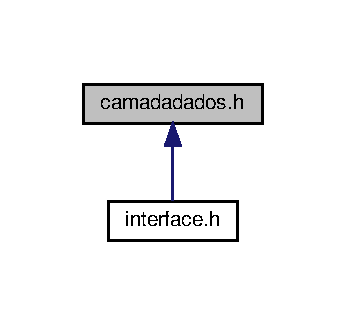
\includegraphics[width=166pt]{camadadados_8h__dep__incl}
\end{center}
\end{figure}
\subsection*{Componentes}
\begin{DoxyCompactItemize}
\item 
struct \hyperlink{structCOORDENADA}{C\+O\+O\+R\+D\+E\+N\+A\+DA}
\begin{DoxyCompactList}\small\item\em Tipo de dados para as coordenadas. \end{DoxyCompactList}\item 
struct \hyperlink{structJOGADA}{J\+O\+G\+A\+DA}
\begin{DoxyCompactList}\small\item\em Tipo de dados para a jogada. \end{DoxyCompactList}\item 
struct \hyperlink{structESTADO}{E\+S\+T\+A\+DO}
\begin{DoxyCompactList}\small\item\em Tipo de dados para o estado. \end{DoxyCompactList}\end{DoxyCompactItemize}
\subsection*{Definições de tipos}
\begin{DoxyCompactItemize}
\item 
\mbox{\Hypertarget{camadadados_8h_a94c221d29a1760f008b7834093259b7d}\label{camadadados_8h_a94c221d29a1760f008b7834093259b7d}} 
typedef \hyperlink{structJOGADA}{J\+O\+G\+A\+DA} \hyperlink{camadadados_8h_a94c221d29a1760f008b7834093259b7d}{J\+O\+G\+A\+D\+AS}\mbox{[}32\mbox{]}
\begin{DoxyCompactList}\small\item\em Tipo de dados para as jogadas. \end{DoxyCompactList}\end{DoxyCompactItemize}
\subsection*{Enumerações}
\begin{DoxyCompactItemize}
\item 
\mbox{\Hypertarget{camadadados_8h_aba91601f16d4c485b2d9b8c429f27039}\label{camadadados_8h_aba91601f16d4c485b2d9b8c429f27039}} 
enum \hyperlink{camadadados_8h_aba91601f16d4c485b2d9b8c429f27039}{C\+A\+SA} \{ \newline
{\bfseries UM} = \textquotesingle{}1\textquotesingle{}, 
{\bfseries D\+O\+IS} = \textquotesingle{}2\textquotesingle{}, 
{\bfseries V\+A\+Z\+IO} = \textquotesingle{}.\textquotesingle{}, 
{\bfseries B\+R\+A\+N\+CA} = \textquotesingle{}$\ast$\textquotesingle{}, 
\newline
{\bfseries P\+R\+E\+TA} = \textquotesingle{}\#\textquotesingle{}
 \}\begin{DoxyCompactList}\small\item\em Tipo de dados para a casa. \end{DoxyCompactList}
\item 
\mbox{\Hypertarget{camadadados_8h_ab8d2e03f1be6ed043ab77a0ea6d0c3fd}\label{camadadados_8h_ab8d2e03f1be6ed043ab77a0ea6d0c3fd}} 
enum \hyperlink{camadadados_8h_ab8d2e03f1be6ed043ab77a0ea6d0c3fd}{E\+R\+R\+OS} \{ \newline
{\bfseries OK}, 
{\bfseries C\+O\+O\+R\+D\+E\+N\+A\+D\+A\+\_\+\+I\+N\+V\+A\+L\+I\+DA}, 
{\bfseries J\+O\+G\+A\+D\+A\+\_\+\+I\+N\+V\+A\+L\+I\+DA}, 
{\bfseries E\+R\+R\+O\+\_\+\+L\+E\+R\+\_\+\+T\+AB}, 
\newline
{\bfseries E\+R\+R\+O\+\_\+\+A\+B\+R\+I\+R\+\_\+\+F\+I\+C\+H\+E\+I\+RO}
 \}\begin{DoxyCompactList}\small\item\em Tipo de dados para os erros. \end{DoxyCompactList}
\end{DoxyCompactItemize}
\subsection*{Funções}
\begin{DoxyCompactItemize}
\item 
\mbox{\Hypertarget{camadadados_8h_a7e0c7e26fb685d9ab501e19b05e6954f}\label{camadadados_8h_a7e0c7e26fb685d9ab501e19b05e6954f}} 
\hyperlink{structESTADO}{E\+S\+T\+A\+DO} $\ast$ \hyperlink{camadadados_8h_a7e0c7e26fb685d9ab501e19b05e6954f}{inicializar\+\_\+estado} ()
\begin{DoxyCompactList}\small\item\em Inicializa um estado. \end{DoxyCompactList}\item 
int \hyperlink{camadadados_8h_a6cd0b387bdee9e18003c78852394aa63}{obter\+\_\+numero\+\_\+de\+\_\+jogadas} (\hyperlink{structESTADO}{E\+S\+T\+A\+DO} $\ast$estado)
\begin{DoxyCompactList}\small\item\em Retorna o número de jogadas. \end{DoxyCompactList}\item 
int \hyperlink{camadadados_8h_af4cf201e91b420cd174888d897512e2d}{conversorultimajogadalinha} (\hyperlink{structCOORDENADA}{C\+O\+O\+R\+D\+E\+N\+A\+DA} c)
\begin{DoxyCompactList}\small\item\em Converte a ultima jogada linha. \end{DoxyCompactList}\item 
char \hyperlink{camadadados_8h_a3c6b8a183e1177d63b9646ff4e9322ac}{conversorultimajogadacoluna} (\hyperlink{structCOORDENADA}{C\+O\+O\+R\+D\+E\+N\+A\+DA} c)
\begin{DoxyCompactList}\small\item\em Converte a ultima jogada coluna. \end{DoxyCompactList}\item 
\hyperlink{camadadados_8h_aba91601f16d4c485b2d9b8c429f27039}{C\+A\+SA} \hyperlink{camadadados_8h_a6faa68373203923729ed38657aa0f768}{obter\+\_\+estado\+\_\+casa} (\hyperlink{structESTADO}{E\+S\+T\+A\+DO} $\ast$e, \hyperlink{structCOORDENADA}{C\+O\+O\+R\+D\+E\+N\+A\+DA} c)
\begin{DoxyCompactList}\small\item\em Obtém o estado da casa. \end{DoxyCompactList}\item 
void \hyperlink{camadadados_8h_a1fc7443b24fac5ea61afbb41f9a00feb}{armazenar\+\_\+jogada} (\hyperlink{structESTADO}{E\+S\+T\+A\+DO} $\ast$e, \hyperlink{structJOGADA}{J\+O\+G\+A\+DA} \hyperlink{logica_8h_a9dfbc982d23a619e36575d8e7ec8e41c}{jog}, int n)
\begin{DoxyCompactList}\small\item\em Funcao que armaneza jogadas. \end{DoxyCompactList}\item 
\hyperlink{structCOORDENADA}{C\+O\+O\+R\+D\+E\+N\+A\+DA} \hyperlink{camadadados_8h_a30d458e0db175363ef23d01614148db5}{get\+\_\+coord\+\_\+jogador1} (\hyperlink{structESTADO}{E\+S\+T\+A\+DO} $\ast$e, int c)
\begin{DoxyCompactList}\small\item\em Funcao para devolver a coordenada do Jogador 1 numa Jogada c. \end{DoxyCompactList}\item 
\hyperlink{structCOORDENADA}{C\+O\+O\+R\+D\+E\+N\+A\+DA} \hyperlink{camadadados_8h_a9f88ef4d79f7afb4ba23c18bcf969b99}{get\+\_\+coord\+\_\+jogador2} (\hyperlink{structESTADO}{E\+S\+T\+A\+DO} $\ast$e, int c)
\begin{DoxyCompactList}\small\item\em Funcao para devolver a coordenada do Jogador 2 numa Jogada c. \end{DoxyCompactList}\item 
int \hyperlink{camadadados_8h_a5bedf93c8d1ff9b665c40b18e6729379}{get\+\_\+coord\+\_\+coluna} (\hyperlink{structCOORDENADA}{C\+O\+O\+R\+D\+E\+N\+A\+DA} c)
\begin{DoxyCompactList}\small\item\em Funcao para devolver a coluna de uma jogada. \end{DoxyCompactList}\item 
void \hyperlink{camadadados_8h_a8828526e2c272cd90636cc20be682929}{altera\+\_\+ultimajogada} (\hyperlink{structESTADO}{E\+S\+T\+A\+DO} $\ast$e, \hyperlink{structCOORDENADA}{C\+O\+O\+R\+D\+E\+N\+A\+DA} c)
\begin{DoxyCompactList}\small\item\em Funcao para alterar a ultima jogada no estado. \end{DoxyCompactList}\item 
void \hyperlink{camadadados_8h_a34423ba176740a47fe988269870dbc42}{set\+\_\+casa} (\hyperlink{structESTADO}{E\+S\+T\+A\+DO} $\ast$e, \hyperlink{structCOORDENADA}{C\+O\+O\+R\+D\+E\+N\+A\+DA} c, \hyperlink{camadadados_8h_aba91601f16d4c485b2d9b8c429f27039}{C\+A\+SA} valor)
\begin{DoxyCompactList}\small\item\em Muda o valor de uma casa. \end{DoxyCompactList}\item 
\hyperlink{structCOORDENADA}{C\+O\+O\+R\+D\+E\+N\+A\+DA} \hyperlink{camadadados_8h_ae89c72e4fa31dcc1eb9ba0fb8ea707e1}{get\+\_\+ultima\+\_\+jogada} (\hyperlink{structESTADO}{E\+S\+T\+A\+DO} $\ast$e)
\begin{DoxyCompactList}\small\item\em Funcao para devolver a coordenada da ultima jogada. \end{DoxyCompactList}\item 
void \hyperlink{camadadados_8h_a3abdb3d91974ec908ad15dac49fa8ed4}{altera\+\_\+estado\+\_\+casa\+\_\+branca} (\hyperlink{structESTADO}{E\+S\+T\+A\+DO} $\ast$e, \hyperlink{structCOORDENADA}{C\+O\+O\+R\+D\+E\+N\+A\+DA} c)
\begin{DoxyCompactList}\small\item\em Funcao para alterar o estado da casa para Branca. \end{DoxyCompactList}\item 
void \hyperlink{camadadados_8h_af2df0559684091c80715656208c7419f}{incrementa\+\_\+numero\+\_\+jogadas} (\hyperlink{structESTADO}{E\+S\+T\+A\+DO} $\ast$e)
\begin{DoxyCompactList}\small\item\em Funcao para incrementar o numero de jogadas. \end{DoxyCompactList}\item 
void \hyperlink{camadadados_8h_a41d8488efb98b187eadb229188da788d}{set\+\_\+jogadas\+\_\+jogador1} (\hyperlink{structESTADO}{E\+S\+T\+A\+DO} $\ast$e, \hyperlink{structCOORDENADA}{C\+O\+O\+R\+D\+E\+N\+A\+DA} c, int n)
\begin{DoxyCompactList}\small\item\em Funcao para inserir uma Jogada do Jogador 1 no estado. \end{DoxyCompactList}\item 
void \hyperlink{camadadados_8h_af90315c6e34540b827b4fdbb10552775}{set\+\_\+jogadas\+\_\+jogador2} (\hyperlink{structESTADO}{E\+S\+T\+A\+DO} $\ast$e, \hyperlink{structCOORDENADA}{C\+O\+O\+R\+D\+E\+N\+A\+DA} c, int n)
\begin{DoxyCompactList}\small\item\em Funcao para inserir uma Jogada do Jogador 2 no estado. \end{DoxyCompactList}\item 
void \hyperlink{camadadados_8h_a2787d03a0237b39a69235b2a1717a34d}{altera\+\_\+estado\+\_\+casa\+\_\+preta} (\hyperlink{structESTADO}{E\+S\+T\+A\+DO} $\ast$e, \hyperlink{structCOORDENADA}{C\+O\+O\+R\+D\+E\+N\+A\+DA} c)
\begin{DoxyCompactList}\small\item\em Funcao para alterar o estado da casa para Preta. \end{DoxyCompactList}\item 
int \hyperlink{camadadados_8h_ab9c95b014d2e217eae7d081088501963}{get\+\_\+jogador\+\_\+atual} (\hyperlink{structESTADO}{E\+S\+T\+A\+DO} $\ast$e)
\begin{DoxyCompactList}\small\item\em Funcao para devolver o Jogador Atual. \end{DoxyCompactList}\item 
void \hyperlink{camadadados_8h_a35c87726f07cb6e89e088c9f2ada6ec2}{set\+\_\+jogador\+\_\+atual} (\hyperlink{structESTADO}{E\+S\+T\+A\+DO} $\ast$e, int x)
\begin{DoxyCompactList}\small\item\em Funcao para alterar o Jogador Atual. \end{DoxyCompactList}\item 
void \hyperlink{camadadados_8h_a2bb319e05de00ed8feb0936e16b7c263}{set\+\_\+jogador\+\_\+vencedor} (\hyperlink{structESTADO}{E\+S\+T\+A\+DO} $\ast$e, int x)
\begin{DoxyCompactList}\small\item\em Funcao para alterar o Vencedor do Jogo. \end{DoxyCompactList}\item 
void \hyperlink{camadadados_8h_a5877b3945165d173d3bdb45d3e5ce333}{set\+\_\+numero\+\_\+jogadas} (\hyperlink{structESTADO}{E\+S\+T\+A\+DO} $\ast$e, int x)
\begin{DoxyCompactList}\small\item\em Funcao para alterar o numero de jogadas. \end{DoxyCompactList}\item 
void \hyperlink{camadadados_8h_a11c86c7543dddcc597997649342ab51e}{altera\+\_\+estado\+\_\+casa\+\_\+vazio} (\hyperlink{structESTADO}{E\+S\+T\+A\+DO} $\ast$e, \hyperlink{structCOORDENADA}{C\+O\+O\+R\+D\+E\+N\+A\+DA} c)
\begin{DoxyCompactList}\small\item\em Funcao para alterar o estada de uma casa para Vazio. \end{DoxyCompactList}\item 
void \hyperlink{camadadados_8h_aa0a6b66d365831c3e507efef17564b86}{altera\+\_\+ultimajogada\+\_\+pos} (\hyperlink{structESTADO}{E\+S\+T\+A\+DO} $\ast$e, int jogada)
\begin{DoxyCompactList}\small\item\em Funcao para alterar as coordenadas da ultima jogada na funcao pos. \end{DoxyCompactList}\item 
\hyperlink{structCOORDENADA}{C\+O\+O\+R\+D\+E\+N\+A\+DA} \hyperlink{camadadados_8h_a65e38a66349ed29267b579412c5cbc53}{get\+\_\+jogadas\+\_\+jogador1} (\hyperlink{structESTADO}{E\+S\+T\+A\+DO} $\ast$e, int n)
\begin{DoxyCompactList}\small\item\em Funcao para obter a Coordenada do Jogador 1 numa certa Jogada. \end{DoxyCompactList}\item 
\hyperlink{structCOORDENADA}{C\+O\+O\+R\+D\+E\+N\+A\+DA} \hyperlink{camadadados_8h_a877bb4d00d7f602710314b2fe8fdb2c8}{get\+\_\+jogadas\+\_\+jogador2} (\hyperlink{structESTADO}{E\+S\+T\+A\+DO} $\ast$e, int n)
\begin{DoxyCompactList}\small\item\em Funcao para obter a Coordenada do Jogador 2 numa certa Jogada. \end{DoxyCompactList}\item 
void \hyperlink{camadadados_8h_a236d410338f232f8434859c40a165205}{set\+\_\+casas\+\_\+invalidas} (\hyperlink{structESTADO}{E\+S\+T\+A\+DO} $\ast$e, int n)
\begin{DoxyCompactList}\small\item\em Funcao para alterar as coordenadas de casas nao utilizadas para -\/1. \end{DoxyCompactList}\item 
int \hyperlink{camadadados_8h_adea30d54df73cf866227a6b6bd790827}{get\+\_\+num\+\_\+jogadas} (\hyperlink{structESTADO}{E\+S\+T\+A\+DO} $\ast$e)
\begin{DoxyCompactList}\small\item\em Funcao para obter o numero de jogadas. \end{DoxyCompactList}\item 
\hyperlink{structESTADO}{E\+S\+T\+A\+DO} $\ast$ \hyperlink{camadadados_8h_ad95b70ad41d5da4f5549b9c839a8d43c}{inicializar\+\_\+estado\+\_\+aux} ()
\begin{DoxyCompactList}\small\item\em Função para inicializar um estado auxiliar que nos permite andar jogadas para a frente na funcao pos. \end{DoxyCompactList}\item 
int \hyperlink{camadadados_8h_a41f8cf8edda55e8622446f79e442ccfa}{get\+\_\+jogador\+\_\+vencedor} (\hyperlink{structESTADO}{E\+S\+T\+A\+DO} $\ast$e)
\begin{DoxyCompactList}\small\item\em Função para obter o jogador vencedor. \end{DoxyCompactList}\item 
void \hyperlink{camadadados_8h_aec75c2e5f40c276d266cf24fdbfe4d24}{set\+\_\+valores} (\hyperlink{structESTADO}{E\+S\+T\+A\+DO} $\ast$e, int valores\mbox{[}8\mbox{]}\mbox{[}8\mbox{]})
\begin{DoxyCompactList}\small\item\em Funcao que atualiza os valores das casas para a floodfill. \end{DoxyCompactList}\item 
int \hyperlink{camadadados_8h_ab30857ddb076ebe58da129e3e7ea7b39}{dentro\+Tabuleiro} (\hyperlink{structCOORDENADA}{C\+O\+O\+R\+D\+E\+N\+A\+DA} c)
\begin{DoxyCompactList}\small\item\em Função que testa se a Coordenada pertence ao Tabuleiro;. \end{DoxyCompactList}\item 
int \hyperlink{camadadados_8h_a33ff7b038dd76f1a6453e8a4b29cb3a8}{get\+\_\+valores} (int valores\mbox{[}8\mbox{]}\mbox{[}8\mbox{]}, \hyperlink{structCOORDENADA}{C\+O\+O\+R\+D\+E\+N\+A\+DA} c)
\begin{DoxyCompactList}\small\item\em Função que devolve o valor de uma coordenada segundo o Algoritmo Flood\+Fill. \end{DoxyCompactList}\end{DoxyCompactItemize}


\subsection{Descrição detalhada}
Definição do estado e das funções que o manipulam 

\subsection{Documentação das funções}
\mbox{\Hypertarget{camadadados_8h_a3abdb3d91974ec908ad15dac49fa8ed4}\label{camadadados_8h_a3abdb3d91974ec908ad15dac49fa8ed4}} 
\index{camadadados.\+h@{camadadados.\+h}!altera\+\_\+estado\+\_\+casa\+\_\+branca@{altera\+\_\+estado\+\_\+casa\+\_\+branca}}
\index{altera\+\_\+estado\+\_\+casa\+\_\+branca@{altera\+\_\+estado\+\_\+casa\+\_\+branca}!camadadados.\+h@{camadadados.\+h}}
\subsubsection{\texorpdfstring{altera\+\_\+estado\+\_\+casa\+\_\+branca()}{altera\_estado\_casa\_branca()}}
{\footnotesize\ttfamily void altera\+\_\+estado\+\_\+casa\+\_\+branca (\begin{DoxyParamCaption}\item[{\hyperlink{structESTADO}{E\+S\+T\+A\+DO} $\ast$}]{e,  }\item[{\hyperlink{structCOORDENADA}{C\+O\+O\+R\+D\+E\+N\+A\+DA}}]{c }\end{DoxyParamCaption})}



Funcao para alterar o estado da casa para Branca. 


\begin{DoxyParams}{Parâmetros}
{\em e} & Apontador para o estado \\
\hline
{\em c} & A coordenada a alterar \\
\hline
\end{DoxyParams}
\mbox{\Hypertarget{camadadados_8h_a2787d03a0237b39a69235b2a1717a34d}\label{camadadados_8h_a2787d03a0237b39a69235b2a1717a34d}} 
\index{camadadados.\+h@{camadadados.\+h}!altera\+\_\+estado\+\_\+casa\+\_\+preta@{altera\+\_\+estado\+\_\+casa\+\_\+preta}}
\index{altera\+\_\+estado\+\_\+casa\+\_\+preta@{altera\+\_\+estado\+\_\+casa\+\_\+preta}!camadadados.\+h@{camadadados.\+h}}
\subsubsection{\texorpdfstring{altera\+\_\+estado\+\_\+casa\+\_\+preta()}{altera\_estado\_casa\_preta()}}
{\footnotesize\ttfamily void altera\+\_\+estado\+\_\+casa\+\_\+preta (\begin{DoxyParamCaption}\item[{\hyperlink{structESTADO}{E\+S\+T\+A\+DO} $\ast$}]{e,  }\item[{\hyperlink{structCOORDENADA}{C\+O\+O\+R\+D\+E\+N\+A\+DA}}]{c }\end{DoxyParamCaption})}



Funcao para alterar o estado da casa para Preta. 


\begin{DoxyParams}{Parâmetros}
{\em e} & Apontador para o estado \\
\hline
{\em c} & A coordenada a alterar \\
\hline
\end{DoxyParams}
\mbox{\Hypertarget{camadadados_8h_a11c86c7543dddcc597997649342ab51e}\label{camadadados_8h_a11c86c7543dddcc597997649342ab51e}} 
\index{camadadados.\+h@{camadadados.\+h}!altera\+\_\+estado\+\_\+casa\+\_\+vazio@{altera\+\_\+estado\+\_\+casa\+\_\+vazio}}
\index{altera\+\_\+estado\+\_\+casa\+\_\+vazio@{altera\+\_\+estado\+\_\+casa\+\_\+vazio}!camadadados.\+h@{camadadados.\+h}}
\subsubsection{\texorpdfstring{altera\+\_\+estado\+\_\+casa\+\_\+vazio()}{altera\_estado\_casa\_vazio()}}
{\footnotesize\ttfamily void altera\+\_\+estado\+\_\+casa\+\_\+vazio (\begin{DoxyParamCaption}\item[{\hyperlink{structESTADO}{E\+S\+T\+A\+DO} $\ast$}]{e,  }\item[{\hyperlink{structCOORDENADA}{C\+O\+O\+R\+D\+E\+N\+A\+DA}}]{c }\end{DoxyParamCaption})}



Funcao para alterar o estada de uma casa para Vazio. 


\begin{DoxyParams}{Parâmetros}
{\em e} & Apontador para o estado \\
\hline
{\em c} & A coordenada da casa a alterar \\
\hline
\end{DoxyParams}
\mbox{\Hypertarget{camadadados_8h_a8828526e2c272cd90636cc20be682929}\label{camadadados_8h_a8828526e2c272cd90636cc20be682929}} 
\index{camadadados.\+h@{camadadados.\+h}!altera\+\_\+ultimajogada@{altera\+\_\+ultimajogada}}
\index{altera\+\_\+ultimajogada@{altera\+\_\+ultimajogada}!camadadados.\+h@{camadadados.\+h}}
\subsubsection{\texorpdfstring{altera\+\_\+ultimajogada()}{altera\_ultimajogada()}}
{\footnotesize\ttfamily void altera\+\_\+ultimajogada (\begin{DoxyParamCaption}\item[{\hyperlink{structESTADO}{E\+S\+T\+A\+DO} $\ast$}]{e,  }\item[{\hyperlink{structCOORDENADA}{C\+O\+O\+R\+D\+E\+N\+A\+DA}}]{c }\end{DoxyParamCaption})}



Funcao para alterar a ultima jogada no estado. 


\begin{DoxyParams}{Parâmetros}
{\em e} & Apontador para o estado \\
\hline
{\em c} & Coordenada a Alterar \\
\hline
\end{DoxyParams}
\mbox{\Hypertarget{camadadados_8h_aa0a6b66d365831c3e507efef17564b86}\label{camadadados_8h_aa0a6b66d365831c3e507efef17564b86}} 
\index{camadadados.\+h@{camadadados.\+h}!altera\+\_\+ultimajogada\+\_\+pos@{altera\+\_\+ultimajogada\+\_\+pos}}
\index{altera\+\_\+ultimajogada\+\_\+pos@{altera\+\_\+ultimajogada\+\_\+pos}!camadadados.\+h@{camadadados.\+h}}
\subsubsection{\texorpdfstring{altera\+\_\+ultimajogada\+\_\+pos()}{altera\_ultimajogada\_pos()}}
{\footnotesize\ttfamily void altera\+\_\+ultimajogada\+\_\+pos (\begin{DoxyParamCaption}\item[{\hyperlink{structESTADO}{E\+S\+T\+A\+DO} $\ast$}]{e,  }\item[{int}]{jogada }\end{DoxyParamCaption})}



Funcao para alterar as coordenadas da ultima jogada na funcao pos. 


\begin{DoxyParams}{Parâmetros}
{\em e} & Apontador para o estado \\
\hline
{\em c} & Inteiro para indicar a Jogada a utilizar \\
\hline
\end{DoxyParams}
\mbox{\Hypertarget{camadadados_8h_a1fc7443b24fac5ea61afbb41f9a00feb}\label{camadadados_8h_a1fc7443b24fac5ea61afbb41f9a00feb}} 
\index{camadadados.\+h@{camadadados.\+h}!armazenar\+\_\+jogada@{armazenar\+\_\+jogada}}
\index{armazenar\+\_\+jogada@{armazenar\+\_\+jogada}!camadadados.\+h@{camadadados.\+h}}
\subsubsection{\texorpdfstring{armazenar\+\_\+jogada()}{armazenar\_jogada()}}
{\footnotesize\ttfamily void armazenar\+\_\+jogada (\begin{DoxyParamCaption}\item[{\hyperlink{structESTADO}{E\+S\+T\+A\+DO} $\ast$}]{e,  }\item[{\hyperlink{structJOGADA}{J\+O\+G\+A\+DA}}]{jog,  }\item[{int}]{n }\end{DoxyParamCaption})}



Funcao que armaneza jogadas. 


\begin{DoxyParams}{Parâmetros}
{\em e} & Apontador para o estado \\
\hline
{\em jog} & Jogada a ser guardada \\
\hline
{\em n} & Número da jogada \\
\hline
\end{DoxyParams}
\mbox{\Hypertarget{camadadados_8h_a3c6b8a183e1177d63b9646ff4e9322ac}\label{camadadados_8h_a3c6b8a183e1177d63b9646ff4e9322ac}} 
\index{camadadados.\+h@{camadadados.\+h}!conversorultimajogadacoluna@{conversorultimajogadacoluna}}
\index{conversorultimajogadacoluna@{conversorultimajogadacoluna}!camadadados.\+h@{camadadados.\+h}}
\subsubsection{\texorpdfstring{conversorultimajogadacoluna()}{conversorultimajogadacoluna()}}
{\footnotesize\ttfamily char conversorultimajogadacoluna (\begin{DoxyParamCaption}\item[{\hyperlink{structCOORDENADA}{C\+O\+O\+R\+D\+E\+N\+A\+DA}}]{c }\end{DoxyParamCaption})}



Converte a ultima jogada coluna. 


\begin{DoxyParams}{Parâmetros}
{\em c} & A coordenada \\
\hline
\end{DoxyParams}
\begin{DoxyReturn}{Retorna}
A coluna da última jogada 
\end{DoxyReturn}
\mbox{\Hypertarget{camadadados_8h_af4cf201e91b420cd174888d897512e2d}\label{camadadados_8h_af4cf201e91b420cd174888d897512e2d}} 
\index{camadadados.\+h@{camadadados.\+h}!conversorultimajogadalinha@{conversorultimajogadalinha}}
\index{conversorultimajogadalinha@{conversorultimajogadalinha}!camadadados.\+h@{camadadados.\+h}}
\subsubsection{\texorpdfstring{conversorultimajogadalinha()}{conversorultimajogadalinha()}}
{\footnotesize\ttfamily int conversorultimajogadalinha (\begin{DoxyParamCaption}\item[{\hyperlink{structCOORDENADA}{C\+O\+O\+R\+D\+E\+N\+A\+DA}}]{c }\end{DoxyParamCaption})}



Converte a ultima jogada linha. 


\begin{DoxyParams}{Parâmetros}
{\em c} & A Coordenada \\
\hline
\end{DoxyParams}
\begin{DoxyReturn}{Retorna}
A linha da última jogada 
\end{DoxyReturn}
\mbox{\Hypertarget{camadadados_8h_ab30857ddb076ebe58da129e3e7ea7b39}\label{camadadados_8h_ab30857ddb076ebe58da129e3e7ea7b39}} 
\index{camadadados.\+h@{camadadados.\+h}!dentro\+Tabuleiro@{dentro\+Tabuleiro}}
\index{dentro\+Tabuleiro@{dentro\+Tabuleiro}!camadadados.\+h@{camadadados.\+h}}
\subsubsection{\texorpdfstring{dentro\+Tabuleiro()}{dentroTabuleiro()}}
{\footnotesize\ttfamily int dentro\+Tabuleiro (\begin{DoxyParamCaption}\item[{\hyperlink{structCOORDENADA}{C\+O\+O\+R\+D\+E\+N\+A\+DA}}]{c }\end{DoxyParamCaption})}



Função que testa se a Coordenada pertence ao Tabuleiro;. 


\begin{DoxyParams}{Parâmetros}
{\em c} & Coordenada \\
\hline
\end{DoxyParams}
\begin{DoxyReturn}{Retorna}
Devolve 1 se está dentro do tabuleiro 
\end{DoxyReturn}
\mbox{\Hypertarget{camadadados_8h_a5bedf93c8d1ff9b665c40b18e6729379}\label{camadadados_8h_a5bedf93c8d1ff9b665c40b18e6729379}} 
\index{camadadados.\+h@{camadadados.\+h}!get\+\_\+coord\+\_\+coluna@{get\+\_\+coord\+\_\+coluna}}
\index{get\+\_\+coord\+\_\+coluna@{get\+\_\+coord\+\_\+coluna}!camadadados.\+h@{camadadados.\+h}}
\subsubsection{\texorpdfstring{get\+\_\+coord\+\_\+coluna()}{get\_coord\_coluna()}}
{\footnotesize\ttfamily int get\+\_\+coord\+\_\+coluna (\begin{DoxyParamCaption}\item[{\hyperlink{structCOORDENADA}{C\+O\+O\+R\+D\+E\+N\+A\+DA}}]{c }\end{DoxyParamCaption})}



Funcao para devolver a coluna de uma jogada. 


\begin{DoxyParams}{Parâmetros}
{\em c} & A coordenada \\
\hline
\end{DoxyParams}
\begin{DoxyReturn}{Retorna}
A coluna 
\end{DoxyReturn}
\mbox{\Hypertarget{camadadados_8h_a30d458e0db175363ef23d01614148db5}\label{camadadados_8h_a30d458e0db175363ef23d01614148db5}} 
\index{camadadados.\+h@{camadadados.\+h}!get\+\_\+coord\+\_\+jogador1@{get\+\_\+coord\+\_\+jogador1}}
\index{get\+\_\+coord\+\_\+jogador1@{get\+\_\+coord\+\_\+jogador1}!camadadados.\+h@{camadadados.\+h}}
\subsubsection{\texorpdfstring{get\+\_\+coord\+\_\+jogador1()}{get\_coord\_jogador1()}}
{\footnotesize\ttfamily \hyperlink{structCOORDENADA}{C\+O\+O\+R\+D\+E\+N\+A\+DA} get\+\_\+coord\+\_\+jogador1 (\begin{DoxyParamCaption}\item[{\hyperlink{structESTADO}{E\+S\+T\+A\+DO} $\ast$}]{e,  }\item[{int}]{c }\end{DoxyParamCaption})}



Funcao para devolver a coordenada do Jogador 1 numa Jogada c. 


\begin{DoxyParams}{Parâmetros}
{\em e} & Apontador para o estado \\
\hline
{\em c} & Numero da Jogada \\
\hline
\end{DoxyParams}
\begin{DoxyReturn}{Retorna}
A Coordenada 
\end{DoxyReturn}
\mbox{\Hypertarget{camadadados_8h_a9f88ef4d79f7afb4ba23c18bcf969b99}\label{camadadados_8h_a9f88ef4d79f7afb4ba23c18bcf969b99}} 
\index{camadadados.\+h@{camadadados.\+h}!get\+\_\+coord\+\_\+jogador2@{get\+\_\+coord\+\_\+jogador2}}
\index{get\+\_\+coord\+\_\+jogador2@{get\+\_\+coord\+\_\+jogador2}!camadadados.\+h@{camadadados.\+h}}
\subsubsection{\texorpdfstring{get\+\_\+coord\+\_\+jogador2()}{get\_coord\_jogador2()}}
{\footnotesize\ttfamily \hyperlink{structCOORDENADA}{C\+O\+O\+R\+D\+E\+N\+A\+DA} get\+\_\+coord\+\_\+jogador2 (\begin{DoxyParamCaption}\item[{\hyperlink{structESTADO}{E\+S\+T\+A\+DO} $\ast$}]{e,  }\item[{int}]{c }\end{DoxyParamCaption})}



Funcao para devolver a coordenada do Jogador 2 numa Jogada c. 


\begin{DoxyParams}{Parâmetros}
{\em e} & Apontador para o estado \\
\hline
{\em c} & Numero da Jogada \\
\hline
\end{DoxyParams}
\begin{DoxyReturn}{Retorna}
A Coordenada 
\end{DoxyReturn}
\mbox{\Hypertarget{camadadados_8h_a65e38a66349ed29267b579412c5cbc53}\label{camadadados_8h_a65e38a66349ed29267b579412c5cbc53}} 
\index{camadadados.\+h@{camadadados.\+h}!get\+\_\+jogadas\+\_\+jogador1@{get\+\_\+jogadas\+\_\+jogador1}}
\index{get\+\_\+jogadas\+\_\+jogador1@{get\+\_\+jogadas\+\_\+jogador1}!camadadados.\+h@{camadadados.\+h}}
\subsubsection{\texorpdfstring{get\+\_\+jogadas\+\_\+jogador1()}{get\_jogadas\_jogador1()}}
{\footnotesize\ttfamily \hyperlink{structCOORDENADA}{C\+O\+O\+R\+D\+E\+N\+A\+DA} get\+\_\+jogadas\+\_\+jogador1 (\begin{DoxyParamCaption}\item[{\hyperlink{structESTADO}{E\+S\+T\+A\+DO} $\ast$}]{e,  }\item[{int}]{n }\end{DoxyParamCaption})}



Funcao para obter a Coordenada do Jogador 1 numa certa Jogada. 


\begin{DoxyParams}{Parâmetros}
{\em e} & Apontador para o estado \\
\hline
{\em n} & Inteiro que indica a Jogada \\
\hline
\end{DoxyParams}
\begin{DoxyReturn}{Retorna}
A coordenada 
\end{DoxyReturn}
\mbox{\Hypertarget{camadadados_8h_a877bb4d00d7f602710314b2fe8fdb2c8}\label{camadadados_8h_a877bb4d00d7f602710314b2fe8fdb2c8}} 
\index{camadadados.\+h@{camadadados.\+h}!get\+\_\+jogadas\+\_\+jogador2@{get\+\_\+jogadas\+\_\+jogador2}}
\index{get\+\_\+jogadas\+\_\+jogador2@{get\+\_\+jogadas\+\_\+jogador2}!camadadados.\+h@{camadadados.\+h}}
\subsubsection{\texorpdfstring{get\+\_\+jogadas\+\_\+jogador2()}{get\_jogadas\_jogador2()}}
{\footnotesize\ttfamily \hyperlink{structCOORDENADA}{C\+O\+O\+R\+D\+E\+N\+A\+DA} get\+\_\+jogadas\+\_\+jogador2 (\begin{DoxyParamCaption}\item[{\hyperlink{structESTADO}{E\+S\+T\+A\+DO} $\ast$}]{e,  }\item[{int}]{n }\end{DoxyParamCaption})}



Funcao para obter a Coordenada do Jogador 2 numa certa Jogada. 


\begin{DoxyParams}{Parâmetros}
{\em e} & Apontador para o estado \\
\hline
{\em n} & Inteiro que indica a Jogada \\
\hline
\end{DoxyParams}
\begin{DoxyReturn}{Retorna}
A coordenada 
\end{DoxyReturn}
\mbox{\Hypertarget{camadadados_8h_ab9c95b014d2e217eae7d081088501963}\label{camadadados_8h_ab9c95b014d2e217eae7d081088501963}} 
\index{camadadados.\+h@{camadadados.\+h}!get\+\_\+jogador\+\_\+atual@{get\+\_\+jogador\+\_\+atual}}
\index{get\+\_\+jogador\+\_\+atual@{get\+\_\+jogador\+\_\+atual}!camadadados.\+h@{camadadados.\+h}}
\subsubsection{\texorpdfstring{get\+\_\+jogador\+\_\+atual()}{get\_jogador\_atual()}}
{\footnotesize\ttfamily int get\+\_\+jogador\+\_\+atual (\begin{DoxyParamCaption}\item[{\hyperlink{structESTADO}{E\+S\+T\+A\+DO} $\ast$}]{e }\end{DoxyParamCaption})}



Funcao para devolver o Jogador Atual. 


\begin{DoxyParams}{Parâmetros}
{\em e} & Apontador para o estado \\
\hline
\end{DoxyParams}
\begin{DoxyReturn}{Retorna}
O jogador atual 
\end{DoxyReturn}
\mbox{\Hypertarget{camadadados_8h_a41f8cf8edda55e8622446f79e442ccfa}\label{camadadados_8h_a41f8cf8edda55e8622446f79e442ccfa}} 
\index{camadadados.\+h@{camadadados.\+h}!get\+\_\+jogador\+\_\+vencedor@{get\+\_\+jogador\+\_\+vencedor}}
\index{get\+\_\+jogador\+\_\+vencedor@{get\+\_\+jogador\+\_\+vencedor}!camadadados.\+h@{camadadados.\+h}}
\subsubsection{\texorpdfstring{get\+\_\+jogador\+\_\+vencedor()}{get\_jogador\_vencedor()}}
{\footnotesize\ttfamily int get\+\_\+jogador\+\_\+vencedor (\begin{DoxyParamCaption}\item[{\hyperlink{structESTADO}{E\+S\+T\+A\+DO} $\ast$}]{e }\end{DoxyParamCaption})}



Função para obter o jogador vencedor. 


\begin{DoxyParams}{Parâmetros}
{\em e} & Apontador para o estado \\
\hline
\end{DoxyParams}
\begin{DoxyReturn}{Retorna}
O jogador vencedor 
\end{DoxyReturn}
\mbox{\Hypertarget{camadadados_8h_adea30d54df73cf866227a6b6bd790827}\label{camadadados_8h_adea30d54df73cf866227a6b6bd790827}} 
\index{camadadados.\+h@{camadadados.\+h}!get\+\_\+num\+\_\+jogadas@{get\+\_\+num\+\_\+jogadas}}
\index{get\+\_\+num\+\_\+jogadas@{get\+\_\+num\+\_\+jogadas}!camadadados.\+h@{camadadados.\+h}}
\subsubsection{\texorpdfstring{get\+\_\+num\+\_\+jogadas()}{get\_num\_jogadas()}}
{\footnotesize\ttfamily int get\+\_\+num\+\_\+jogadas (\begin{DoxyParamCaption}\item[{\hyperlink{structESTADO}{E\+S\+T\+A\+DO} $\ast$}]{e }\end{DoxyParamCaption})}



Funcao para obter o numero de jogadas. 


\begin{DoxyParams}{Parâmetros}
{\em e} & Apontador para o estado \\
\hline
\end{DoxyParams}
\begin{DoxyReturn}{Retorna}
O número de jogadas 
\end{DoxyReturn}
\mbox{\Hypertarget{camadadados_8h_ae89c72e4fa31dcc1eb9ba0fb8ea707e1}\label{camadadados_8h_ae89c72e4fa31dcc1eb9ba0fb8ea707e1}} 
\index{camadadados.\+h@{camadadados.\+h}!get\+\_\+ultima\+\_\+jogada@{get\+\_\+ultima\+\_\+jogada}}
\index{get\+\_\+ultima\+\_\+jogada@{get\+\_\+ultima\+\_\+jogada}!camadadados.\+h@{camadadados.\+h}}
\subsubsection{\texorpdfstring{get\+\_\+ultima\+\_\+jogada()}{get\_ultima\_jogada()}}
{\footnotesize\ttfamily \hyperlink{structCOORDENADA}{C\+O\+O\+R\+D\+E\+N\+A\+DA} get\+\_\+ultima\+\_\+jogada (\begin{DoxyParamCaption}\item[{\hyperlink{structESTADO}{E\+S\+T\+A\+DO} $\ast$}]{e }\end{DoxyParamCaption})}



Funcao para devolver a coordenada da ultima jogada. 


\begin{DoxyParams}{Parâmetros}
{\em e} & Apontador para o estado \\
\hline
\end{DoxyParams}
\begin{DoxyReturn}{Retorna}
A Coordenada 
\end{DoxyReturn}
\mbox{\Hypertarget{camadadados_8h_a33ff7b038dd76f1a6453e8a4b29cb3a8}\label{camadadados_8h_a33ff7b038dd76f1a6453e8a4b29cb3a8}} 
\index{camadadados.\+h@{camadadados.\+h}!get\+\_\+valores@{get\+\_\+valores}}
\index{get\+\_\+valores@{get\+\_\+valores}!camadadados.\+h@{camadadados.\+h}}
\subsubsection{\texorpdfstring{get\+\_\+valores()}{get\_valores()}}
{\footnotesize\ttfamily int get\+\_\+valores (\begin{DoxyParamCaption}\item[{int}]{valores\mbox{[}8\mbox{]}\mbox{[}8\mbox{]},  }\item[{\hyperlink{structCOORDENADA}{C\+O\+O\+R\+D\+E\+N\+A\+DA}}]{c }\end{DoxyParamCaption})}



Função que devolve o valor de uma coordenada segundo o Algoritmo Flood\+Fill. 


\begin{DoxyParams}{Parâmetros}
{\em valores} & Matriz de Valores \\
\hline
{\em c} & Coordenada \\
\hline
\end{DoxyParams}
\begin{DoxyReturn}{Retorna}
Valor da Coordenada 
\end{DoxyReturn}
\mbox{\Hypertarget{camadadados_8h_af2df0559684091c80715656208c7419f}\label{camadadados_8h_af2df0559684091c80715656208c7419f}} 
\index{camadadados.\+h@{camadadados.\+h}!incrementa\+\_\+numero\+\_\+jogadas@{incrementa\+\_\+numero\+\_\+jogadas}}
\index{incrementa\+\_\+numero\+\_\+jogadas@{incrementa\+\_\+numero\+\_\+jogadas}!camadadados.\+h@{camadadados.\+h}}
\subsubsection{\texorpdfstring{incrementa\+\_\+numero\+\_\+jogadas()}{incrementa\_numero\_jogadas()}}
{\footnotesize\ttfamily void incrementa\+\_\+numero\+\_\+jogadas (\begin{DoxyParamCaption}\item[{\hyperlink{structESTADO}{E\+S\+T\+A\+DO} $\ast$}]{e }\end{DoxyParamCaption})}



Funcao para incrementar o numero de jogadas. 


\begin{DoxyParams}{Parâmetros}
{\em e} & Apontador para o estado \\
\hline
\end{DoxyParams}
\mbox{\Hypertarget{camadadados_8h_ad95b70ad41d5da4f5549b9c839a8d43c}\label{camadadados_8h_ad95b70ad41d5da4f5549b9c839a8d43c}} 
\index{camadadados.\+h@{camadadados.\+h}!inicializar\+\_\+estado\+\_\+aux@{inicializar\+\_\+estado\+\_\+aux}}
\index{inicializar\+\_\+estado\+\_\+aux@{inicializar\+\_\+estado\+\_\+aux}!camadadados.\+h@{camadadados.\+h}}
\subsubsection{\texorpdfstring{inicializar\+\_\+estado\+\_\+aux()}{inicializar\_estado\_aux()}}
{\footnotesize\ttfamily \hyperlink{structESTADO}{E\+S\+T\+A\+DO}$\ast$ inicializar\+\_\+estado\+\_\+aux (\begin{DoxyParamCaption}{ }\end{DoxyParamCaption})}



Função para inicializar um estado auxiliar que nos permite andar jogadas para a frente na funcao pos. 

\begin{DoxyReturn}{Retorna}
O novo estado 
\end{DoxyReturn}
\mbox{\Hypertarget{camadadados_8h_a6faa68373203923729ed38657aa0f768}\label{camadadados_8h_a6faa68373203923729ed38657aa0f768}} 
\index{camadadados.\+h@{camadadados.\+h}!obter\+\_\+estado\+\_\+casa@{obter\+\_\+estado\+\_\+casa}}
\index{obter\+\_\+estado\+\_\+casa@{obter\+\_\+estado\+\_\+casa}!camadadados.\+h@{camadadados.\+h}}
\subsubsection{\texorpdfstring{obter\+\_\+estado\+\_\+casa()}{obter\_estado\_casa()}}
{\footnotesize\ttfamily \hyperlink{camadadados_8h_aba91601f16d4c485b2d9b8c429f27039}{C\+A\+SA} obter\+\_\+estado\+\_\+casa (\begin{DoxyParamCaption}\item[{\hyperlink{structESTADO}{E\+S\+T\+A\+DO} $\ast$}]{e,  }\item[{\hyperlink{structCOORDENADA}{C\+O\+O\+R\+D\+E\+N\+A\+DA}}]{c }\end{DoxyParamCaption})}



Obtém o estado da casa. 


\begin{DoxyParams}{Parâmetros}
{\em e} & Apontador para o estado \\
\hline
{\em c} & A coordenada \\
\hline
\end{DoxyParams}
\begin{DoxyReturn}{Retorna}
O estado da casa 
\end{DoxyReturn}
\mbox{\Hypertarget{camadadados_8h_a6cd0b387bdee9e18003c78852394aa63}\label{camadadados_8h_a6cd0b387bdee9e18003c78852394aa63}} 
\index{camadadados.\+h@{camadadados.\+h}!obter\+\_\+numero\+\_\+de\+\_\+jogadas@{obter\+\_\+numero\+\_\+de\+\_\+jogadas}}
\index{obter\+\_\+numero\+\_\+de\+\_\+jogadas@{obter\+\_\+numero\+\_\+de\+\_\+jogadas}!camadadados.\+h@{camadadados.\+h}}
\subsubsection{\texorpdfstring{obter\+\_\+numero\+\_\+de\+\_\+jogadas()}{obter\_numero\_de\_jogadas()}}
{\footnotesize\ttfamily int obter\+\_\+numero\+\_\+de\+\_\+jogadas (\begin{DoxyParamCaption}\item[{\hyperlink{structESTADO}{E\+S\+T\+A\+DO} $\ast$}]{estado }\end{DoxyParamCaption})}



Retorna o número de jogadas. 


\begin{DoxyParams}{Parâmetros}
{\em estado} & Apontador para o estado \\
\hline
\end{DoxyParams}
\begin{DoxyReturn}{Retorna}
O número de jogadas 
\end{DoxyReturn}
\mbox{\Hypertarget{camadadados_8h_a34423ba176740a47fe988269870dbc42}\label{camadadados_8h_a34423ba176740a47fe988269870dbc42}} 
\index{camadadados.\+h@{camadadados.\+h}!set\+\_\+casa@{set\+\_\+casa}}
\index{set\+\_\+casa@{set\+\_\+casa}!camadadados.\+h@{camadadados.\+h}}
\subsubsection{\texorpdfstring{set\+\_\+casa()}{set\_casa()}}
{\footnotesize\ttfamily void set\+\_\+casa (\begin{DoxyParamCaption}\item[{\hyperlink{structESTADO}{E\+S\+T\+A\+DO} $\ast$}]{e,  }\item[{\hyperlink{structCOORDENADA}{C\+O\+O\+R\+D\+E\+N\+A\+DA}}]{c,  }\item[{\hyperlink{camadadados_8h_aba91601f16d4c485b2d9b8c429f27039}{C\+A\+SA}}]{valor }\end{DoxyParamCaption})}



Muda o valor de uma casa. 


\begin{DoxyParams}{Parâmetros}
{\em e} & Apontador para o estado \\
\hline
{\em c} & A coordenada \\
\hline
{\em V} & O novo valor para a casa \\
\hline
\end{DoxyParams}
\mbox{\Hypertarget{camadadados_8h_a236d410338f232f8434859c40a165205}\label{camadadados_8h_a236d410338f232f8434859c40a165205}} 
\index{camadadados.\+h@{camadadados.\+h}!set\+\_\+casas\+\_\+invalidas@{set\+\_\+casas\+\_\+invalidas}}
\index{set\+\_\+casas\+\_\+invalidas@{set\+\_\+casas\+\_\+invalidas}!camadadados.\+h@{camadadados.\+h}}
\subsubsection{\texorpdfstring{set\+\_\+casas\+\_\+invalidas()}{set\_casas\_invalidas()}}
{\footnotesize\ttfamily void set\+\_\+casas\+\_\+invalidas (\begin{DoxyParamCaption}\item[{\hyperlink{structESTADO}{E\+S\+T\+A\+DO} $\ast$}]{e,  }\item[{int}]{n }\end{DoxyParamCaption})}



Funcao para alterar as coordenadas de casas nao utilizadas para -\/1. 


\begin{DoxyParams}{Parâmetros}
{\em e} & Apontador para o estado \\
\hline
{\em c} & Inteiro que indica a Jogada a alterar \\
\hline
\end{DoxyParams}
\mbox{\Hypertarget{camadadados_8h_a41d8488efb98b187eadb229188da788d}\label{camadadados_8h_a41d8488efb98b187eadb229188da788d}} 
\index{camadadados.\+h@{camadadados.\+h}!set\+\_\+jogadas\+\_\+jogador1@{set\+\_\+jogadas\+\_\+jogador1}}
\index{set\+\_\+jogadas\+\_\+jogador1@{set\+\_\+jogadas\+\_\+jogador1}!camadadados.\+h@{camadadados.\+h}}
\subsubsection{\texorpdfstring{set\+\_\+jogadas\+\_\+jogador1()}{set\_jogadas\_jogador1()}}
{\footnotesize\ttfamily void set\+\_\+jogadas\+\_\+jogador1 (\begin{DoxyParamCaption}\item[{\hyperlink{structESTADO}{E\+S\+T\+A\+DO} $\ast$}]{e,  }\item[{\hyperlink{structCOORDENADA}{C\+O\+O\+R\+D\+E\+N\+A\+DA}}]{c,  }\item[{int}]{n }\end{DoxyParamCaption})}



Funcao para inserir uma Jogada do Jogador 1 no estado. 


\begin{DoxyParams}{Parâmetros}
{\em e} & Apontador para o estado \\
\hline
{\em c} & A coordenada a inserir \\
\hline
{\em n} & Numero da Jogada \\
\hline
\end{DoxyParams}
\mbox{\Hypertarget{camadadados_8h_af90315c6e34540b827b4fdbb10552775}\label{camadadados_8h_af90315c6e34540b827b4fdbb10552775}} 
\index{camadadados.\+h@{camadadados.\+h}!set\+\_\+jogadas\+\_\+jogador2@{set\+\_\+jogadas\+\_\+jogador2}}
\index{set\+\_\+jogadas\+\_\+jogador2@{set\+\_\+jogadas\+\_\+jogador2}!camadadados.\+h@{camadadados.\+h}}
\subsubsection{\texorpdfstring{set\+\_\+jogadas\+\_\+jogador2()}{set\_jogadas\_jogador2()}}
{\footnotesize\ttfamily void set\+\_\+jogadas\+\_\+jogador2 (\begin{DoxyParamCaption}\item[{\hyperlink{structESTADO}{E\+S\+T\+A\+DO} $\ast$}]{e,  }\item[{\hyperlink{structCOORDENADA}{C\+O\+O\+R\+D\+E\+N\+A\+DA}}]{c,  }\item[{int}]{n }\end{DoxyParamCaption})}



Funcao para inserir uma Jogada do Jogador 2 no estado. 


\begin{DoxyParams}{Parâmetros}
{\em e} & Apontador para o estado \\
\hline
{\em c} & A coordenada a inserir \\
\hline
{\em n} & Numero da Jogada \\
\hline
\end{DoxyParams}
\mbox{\Hypertarget{camadadados_8h_a35c87726f07cb6e89e088c9f2ada6ec2}\label{camadadados_8h_a35c87726f07cb6e89e088c9f2ada6ec2}} 
\index{camadadados.\+h@{camadadados.\+h}!set\+\_\+jogador\+\_\+atual@{set\+\_\+jogador\+\_\+atual}}
\index{set\+\_\+jogador\+\_\+atual@{set\+\_\+jogador\+\_\+atual}!camadadados.\+h@{camadadados.\+h}}
\subsubsection{\texorpdfstring{set\+\_\+jogador\+\_\+atual()}{set\_jogador\_atual()}}
{\footnotesize\ttfamily void set\+\_\+jogador\+\_\+atual (\begin{DoxyParamCaption}\item[{\hyperlink{structESTADO}{E\+S\+T\+A\+DO} $\ast$}]{e,  }\item[{int}]{x }\end{DoxyParamCaption})}



Funcao para alterar o Jogador Atual. 


\begin{DoxyParams}{Parâmetros}
{\em e} & Apontador para o estado \\
\hline
{\em x} & Jogador a Alterar \\
\hline
\end{DoxyParams}
\mbox{\Hypertarget{camadadados_8h_a2bb319e05de00ed8feb0936e16b7c263}\label{camadadados_8h_a2bb319e05de00ed8feb0936e16b7c263}} 
\index{camadadados.\+h@{camadadados.\+h}!set\+\_\+jogador\+\_\+vencedor@{set\+\_\+jogador\+\_\+vencedor}}
\index{set\+\_\+jogador\+\_\+vencedor@{set\+\_\+jogador\+\_\+vencedor}!camadadados.\+h@{camadadados.\+h}}
\subsubsection{\texorpdfstring{set\+\_\+jogador\+\_\+vencedor()}{set\_jogador\_vencedor()}}
{\footnotesize\ttfamily void set\+\_\+jogador\+\_\+vencedor (\begin{DoxyParamCaption}\item[{\hyperlink{structESTADO}{E\+S\+T\+A\+DO} $\ast$}]{e,  }\item[{int}]{x }\end{DoxyParamCaption})}



Funcao para alterar o Vencedor do Jogo. 


\begin{DoxyParams}{Parâmetros}
{\em e} & Apontador para o estado \\
\hline
{\em c} & O Vencedor \\
\hline
\end{DoxyParams}
\mbox{\Hypertarget{camadadados_8h_a5877b3945165d173d3bdb45d3e5ce333}\label{camadadados_8h_a5877b3945165d173d3bdb45d3e5ce333}} 
\index{camadadados.\+h@{camadadados.\+h}!set\+\_\+numero\+\_\+jogadas@{set\+\_\+numero\+\_\+jogadas}}
\index{set\+\_\+numero\+\_\+jogadas@{set\+\_\+numero\+\_\+jogadas}!camadadados.\+h@{camadadados.\+h}}
\subsubsection{\texorpdfstring{set\+\_\+numero\+\_\+jogadas()}{set\_numero\_jogadas()}}
{\footnotesize\ttfamily void set\+\_\+numero\+\_\+jogadas (\begin{DoxyParamCaption}\item[{\hyperlink{structESTADO}{E\+S\+T\+A\+DO} $\ast$}]{e,  }\item[{int}]{x }\end{DoxyParamCaption})}



Funcao para alterar o numero de jogadas. 


\begin{DoxyParams}{Parâmetros}
{\em e} & Apontador para o estado \\
\hline
{\em c} & Numero de Jogadas a alterar \\
\hline
\end{DoxyParams}
\mbox{\Hypertarget{camadadados_8h_aec75c2e5f40c276d266cf24fdbfe4d24}\label{camadadados_8h_aec75c2e5f40c276d266cf24fdbfe4d24}} 
\index{camadadados.\+h@{camadadados.\+h}!set\+\_\+valores@{set\+\_\+valores}}
\index{set\+\_\+valores@{set\+\_\+valores}!camadadados.\+h@{camadadados.\+h}}
\subsubsection{\texorpdfstring{set\+\_\+valores()}{set\_valores()}}
{\footnotesize\ttfamily void set\+\_\+valores (\begin{DoxyParamCaption}\item[{\hyperlink{structESTADO}{E\+S\+T\+A\+DO} $\ast$}]{e,  }\item[{int}]{valores\mbox{[}8\mbox{]}\mbox{[}8\mbox{]} }\end{DoxyParamCaption})}



Funcao que atualiza os valores das casas para a floodfill. 


\begin{DoxyParams}{Parâmetros}
{\em e} & Apontador para o estado \\
\hline
{\em valores} & Valores do tabuleiro \\
\hline
\end{DoxyParams}

\hypertarget{interface_8h}{}\section{Referência ao ficheiro interface.\+h}
\label{interface_8h}\index{interface.\+h@{interface.\+h}}
{\ttfamily \#include \char`\"{}camadadados.\+h\char`\"{}}\newline
Diagrama de dependências de inclusão para interface.\+h\+:
% FIG 0
\subsection*{Funções}
\begin{DoxyCompactItemize}
\item 
void \hyperlink{interface_8h_acbc064f5e208515bc1b58b731cc17c94}{movimentos} (\hyperlink{structESTADO}{E\+S\+T\+A\+DO} $\ast$e)
\begin{DoxyCompactList}\small\item\em Funcao que imprime as jogadas no ecrã. \end{DoxyCompactList}\item 
void \hyperlink{interface_8h_a4525a57d0cd9ed3c9150e19b67e1dad6}{mostrar\+\_\+tabuleiro} (\hyperlink{structESTADO}{E\+S\+T\+A\+DO} $\ast$estado)
\begin{DoxyCompactList}\small\item\em Função que mostra o tabuleiro. \end{DoxyCompactList}\item 
\hyperlink{camadadados_8h_ab8d2e03f1be6ed043ab77a0ea6d0c3fd}{E\+R\+R\+OS} \hyperlink{interface_8h_a8fc889059d5c36644fbc1665d750984f}{gravar} (\hyperlink{structESTADO}{E\+S\+T\+A\+DO} $\ast$e, char $\ast$ficheiro)
\begin{DoxyCompactList}\small\item\em Grava o estado do tabuleiro. \end{DoxyCompactList}\item 
\hyperlink{camadadados_8h_ab8d2e03f1be6ed043ab77a0ea6d0c3fd}{E\+R\+R\+OS} \hyperlink{interface_8h_ab752e7aff17a25212d714bd5f8c7fb12}{ler} (\hyperlink{structESTADO}{E\+S\+T\+A\+DO} $\ast$e, char $\ast$ficheiro)
\begin{DoxyCompactList}\small\item\em Função que faz a leitura do tabuleiro. \end{DoxyCompactList}\item 
void \hyperlink{interface_8h_ab2fb8cd7bf019ed1c45b7987033795dd}{jogar} (\hyperlink{structESTADO}{E\+S\+T\+A\+DO} $\ast$estado, \hyperlink{structCOORDENADA}{C\+O\+O\+R\+D\+E\+N\+A\+DA} c)
\begin{DoxyCompactList}\small\item\em Função principal que efetua a jogada. \end{DoxyCompactList}\item 
int \hyperlink{interface_8h_a31caa50aca7bd50a3c62db5b2316108a}{interpretador} (\hyperlink{structESTADO}{E\+S\+T\+A\+DO} $\ast$e, \hyperlink{structESTADO}{E\+S\+T\+A\+DO} $\ast$aux)
\begin{DoxyCompactList}\small\item\em Interpretador de comandos. \end{DoxyCompactList}\end{DoxyCompactItemize}


\subsection{Descrição detalhada}
Interpretador e funcões complementares a este. 

\subsection{Documentação das funções}
\mbox{\Hypertarget{interface_8h_a8fc889059d5c36644fbc1665d750984f}\label{interface_8h_a8fc889059d5c36644fbc1665d750984f}} 
\index{interface.\+h@{interface.\+h}!gravar@{gravar}}
\index{gravar@{gravar}!interface.\+h@{interface.\+h}}
\subsubsection{\texorpdfstring{gravar()}{gravar()}}
{\footnotesize\ttfamily \hyperlink{camadadados_8h_ab8d2e03f1be6ed043ab77a0ea6d0c3fd}{E\+R\+R\+OS} gravar (\begin{DoxyParamCaption}\item[{\hyperlink{structESTADO}{E\+S\+T\+A\+DO} $\ast$}]{e,  }\item[{char $\ast$}]{ficheiro }\end{DoxyParamCaption})}



Grava o estado do tabuleiro. 


\begin{DoxyParams}{Parâmetros}
{\em e} & Apontador para o estado \\
\hline
{\em ficheiro} & Apontador para o nome do ficheiro \\
\hline
\end{DoxyParams}
\begin{DoxyReturn}{Retorna}
Devolve OK se conseguiu gravar 
\end{DoxyReturn}
\mbox{\Hypertarget{interface_8h_a31caa50aca7bd50a3c62db5b2316108a}\label{interface_8h_a31caa50aca7bd50a3c62db5b2316108a}} 
\index{interface.\+h@{interface.\+h}!interpretador@{interpretador}}
\index{interpretador@{interpretador}!interface.\+h@{interface.\+h}}
\subsubsection{\texorpdfstring{interpretador()}{interpretador()}}
{\footnotesize\ttfamily int interpretador (\begin{DoxyParamCaption}\item[{\hyperlink{structESTADO}{E\+S\+T\+A\+DO} $\ast$}]{e,  }\item[{\hyperlink{structESTADO}{E\+S\+T\+A\+DO} $\ast$}]{aux }\end{DoxyParamCaption})}



Interpretador de comandos. 


\begin{DoxyParams}{Parâmetros}
{\em e} & Apontador para o estado \\
\hline
\end{DoxyParams}
\begin{DoxyReturn}{Retorna}
Devolve 1 no final do programa 
\end{DoxyReturn}
\mbox{\Hypertarget{interface_8h_ab2fb8cd7bf019ed1c45b7987033795dd}\label{interface_8h_ab2fb8cd7bf019ed1c45b7987033795dd}} 
\index{interface.\+h@{interface.\+h}!jogar@{jogar}}
\index{jogar@{jogar}!interface.\+h@{interface.\+h}}
\subsubsection{\texorpdfstring{jogar()}{jogar()}}
{\footnotesize\ttfamily void jogar (\begin{DoxyParamCaption}\item[{\hyperlink{structESTADO}{E\+S\+T\+A\+DO} $\ast$}]{estado,  }\item[{\hyperlink{structCOORDENADA}{C\+O\+O\+R\+D\+E\+N\+A\+DA}}]{c }\end{DoxyParamCaption})}



Função principal que efetua a jogada. 


\begin{DoxyParams}{Parâmetros}
{\em estado} & Apontador para o estado \\
\hline
{\em c} & A coordenada \\
\hline
\end{DoxyParams}
\mbox{\Hypertarget{interface_8h_ab752e7aff17a25212d714bd5f8c7fb12}\label{interface_8h_ab752e7aff17a25212d714bd5f8c7fb12}} 
\index{interface.\+h@{interface.\+h}!ler@{ler}}
\index{ler@{ler}!interface.\+h@{interface.\+h}}
\subsubsection{\texorpdfstring{ler()}{ler()}}
{\footnotesize\ttfamily \hyperlink{camadadados_8h_ab8d2e03f1be6ed043ab77a0ea6d0c3fd}{E\+R\+R\+OS} ler (\begin{DoxyParamCaption}\item[{\hyperlink{structESTADO}{E\+S\+T\+A\+DO} $\ast$}]{e,  }\item[{char $\ast$}]{ficheiro }\end{DoxyParamCaption})}



Função que faz a leitura do tabuleiro. 


\begin{DoxyParams}{Parâmetros}
{\em e} & Apontador para o estado \\
\hline
{\em ficheiro} & Apontador para o nome do ficheiro \\
\hline
\end{DoxyParams}
\begin{DoxyReturn}{Retorna}
Devolve OK se conseguiu ler 
\end{DoxyReturn}
\mbox{\Hypertarget{interface_8h_a4525a57d0cd9ed3c9150e19b67e1dad6}\label{interface_8h_a4525a57d0cd9ed3c9150e19b67e1dad6}} 
\index{interface.\+h@{interface.\+h}!mostrar\+\_\+tabuleiro@{mostrar\+\_\+tabuleiro}}
\index{mostrar\+\_\+tabuleiro@{mostrar\+\_\+tabuleiro}!interface.\+h@{interface.\+h}}
\subsubsection{\texorpdfstring{mostrar\+\_\+tabuleiro()}{mostrar\_tabuleiro()}}
{\footnotesize\ttfamily void mostrar\+\_\+tabuleiro (\begin{DoxyParamCaption}\item[{\hyperlink{structESTADO}{E\+S\+T\+A\+DO} $\ast$}]{estado }\end{DoxyParamCaption})}



Função que mostra o tabuleiro. 


\begin{DoxyParams}{Parâmetros}
{\em estado} & O estado \\
\hline
\end{DoxyParams}
\mbox{\Hypertarget{interface_8h_acbc064f5e208515bc1b58b731cc17c94}\label{interface_8h_acbc064f5e208515bc1b58b731cc17c94}} 
\index{interface.\+h@{interface.\+h}!movimentos@{movimentos}}
\index{movimentos@{movimentos}!interface.\+h@{interface.\+h}}
\subsubsection{\texorpdfstring{movimentos()}{movimentos()}}
{\footnotesize\ttfamily void movimentos (\begin{DoxyParamCaption}\item[{\hyperlink{structESTADO}{E\+S\+T\+A\+DO} $\ast$}]{e }\end{DoxyParamCaption})}



Funcao que imprime as jogadas no ecrã. 


\begin{DoxyParams}{Parâmetros}
{\em e} & Apontador para o ficheiro \\
\hline
\end{DoxyParams}

\hypertarget{lista_8h}{}\section{Referência ao ficheiro lista.\+h}
\label{lista_8h}\index{lista.\+h@{lista.\+h}}
Este grafo mostra quais são os ficheiros que incluem directamente ou indirectamente este ficheiro\+:\nopagebreak
\begin{figure}[H]
\begin{center}
\leavevmode
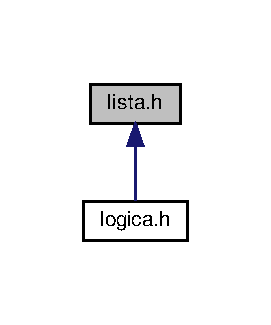
\includegraphics[width=130pt]{lista_8h__dep__incl}
\end{center}
\end{figure}
\subsection*{Componentes}
\begin{DoxyCompactItemize}
\item 
struct \hyperlink{structnodo}{nodo}
\begin{DoxyCompactList}\small\item\em Tipo de dados para as listas ligadas. \end{DoxyCompactList}\end{DoxyCompactItemize}
\subsection*{Definições de tipos}
\begin{DoxyCompactItemize}
\item 
\mbox{\Hypertarget{lista_8h_ac83cdfd19a10fa3718a0707a58732ee1}\label{lista_8h_ac83cdfd19a10fa3718a0707a58732ee1}} 
typedef struct \hyperlink{structnodo}{nodo} \hyperlink{lista_8h_ac83cdfd19a10fa3718a0707a58732ee1}{Nodo}
\begin{DoxyCompactList}\small\item\em Tipo de dados para as listas ligadas. \end{DoxyCompactList}\item 
\mbox{\Hypertarget{lista_8h_a2ed03b19209dd10718380b31b09a69f5}\label{lista_8h_a2ed03b19209dd10718380b31b09a69f5}} 
typedef struct \hyperlink{structnodo}{nodo} $\ast$ {\bfseries L\+I\+S\+TA}
\end{DoxyCompactItemize}
\subsection*{Funções}
\begin{DoxyCompactItemize}
\item 
\hyperlink{structnodo}{L\+I\+S\+TA} \hyperlink{lista_8h_ae3b99323b6f8f35d80bb69ff1a27985e}{criar\+\_\+lista} ()
\begin{DoxyCompactList}\small\item\em Função que cria uma lista ligada. \end{DoxyCompactList}\item 
\hyperlink{structnodo}{L\+I\+S\+TA} \hyperlink{lista_8h_a37ba5fc3cfddb6bc94d4b54b00bc696e}{insere\+\_\+cabeca} (\hyperlink{structnodo}{L\+I\+S\+TA} L, void $\ast$valor)
\begin{DoxyCompactList}\small\item\em Função que insere um nodo no ínicio da lista. \end{DoxyCompactList}\item 
void $\ast$ \hyperlink{lista_8h_abfcb205f3eb670157be0d1221021714b}{devolve\+\_\+cabeca} (\hyperlink{structnodo}{L\+I\+S\+TA} L)
\begin{DoxyCompactList}\small\item\em Função que devolve a cabeça da lista. \end{DoxyCompactList}\item 
\hyperlink{structnodo}{L\+I\+S\+TA} \hyperlink{lista_8h_ad9380152361127432c55c1c6067e05ae}{proximo} (\hyperlink{structnodo}{L\+I\+S\+TA} L)
\begin{DoxyCompactList}\small\item\em Função que insere um nodo no ínicio da lista. \end{DoxyCompactList}\item 
\hyperlink{structnodo}{L\+I\+S\+TA} \hyperlink{lista_8h_a9026a681a68322b5ec7f07137b864cbd}{remove\+\_\+cabeca} (\hyperlink{structnodo}{L\+I\+S\+TA} L)
\begin{DoxyCompactList}\small\item\em Função que remove a cabeça da lista e devolve a cauda. \end{DoxyCompactList}\item 
int \hyperlink{lista_8h_a4c10928f7acaa4e3de3760cea0dfd9c0}{lista\+\_\+esta\+\_\+vazia} (\hyperlink{structnodo}{L\+I\+S\+TA} L)
\begin{DoxyCompactList}\small\item\em Função que verifica se a lista está vazia. \end{DoxyCompactList}\end{DoxyCompactItemize}


\subsection{Descrição detalhada}
Funções para utilizar listas ligadas 

\subsection{Documentação das funções}
\mbox{\Hypertarget{lista_8h_ae3b99323b6f8f35d80bb69ff1a27985e}\label{lista_8h_ae3b99323b6f8f35d80bb69ff1a27985e}} 
\index{lista.\+h@{lista.\+h}!criar\+\_\+lista@{criar\+\_\+lista}}
\index{criar\+\_\+lista@{criar\+\_\+lista}!lista.\+h@{lista.\+h}}
\subsubsection{\texorpdfstring{criar\+\_\+lista()}{criar\_lista()}}
{\footnotesize\ttfamily \hyperlink{structnodo}{L\+I\+S\+TA} criar\+\_\+lista (\begin{DoxyParamCaption}{ }\end{DoxyParamCaption})}



Função que cria uma lista ligada. 

\begin{DoxyReturn}{Retorna}
A lista criada 
\end{DoxyReturn}
\mbox{\Hypertarget{lista_8h_abfcb205f3eb670157be0d1221021714b}\label{lista_8h_abfcb205f3eb670157be0d1221021714b}} 
\index{lista.\+h@{lista.\+h}!devolve\+\_\+cabeca@{devolve\+\_\+cabeca}}
\index{devolve\+\_\+cabeca@{devolve\+\_\+cabeca}!lista.\+h@{lista.\+h}}
\subsubsection{\texorpdfstring{devolve\+\_\+cabeca()}{devolve\_cabeca()}}
{\footnotesize\ttfamily void$\ast$ devolve\+\_\+cabeca (\begin{DoxyParamCaption}\item[{\hyperlink{structnodo}{L\+I\+S\+TA}}]{L }\end{DoxyParamCaption})}



Função que devolve a cabeça da lista. 


\begin{DoxyParams}{Parâmetros}
{\em l} & Lista ligada \\
\hline
\end{DoxyParams}
\mbox{\Hypertarget{lista_8h_a37ba5fc3cfddb6bc94d4b54b00bc696e}\label{lista_8h_a37ba5fc3cfddb6bc94d4b54b00bc696e}} 
\index{lista.\+h@{lista.\+h}!insere\+\_\+cabeca@{insere\+\_\+cabeca}}
\index{insere\+\_\+cabeca@{insere\+\_\+cabeca}!lista.\+h@{lista.\+h}}
\subsubsection{\texorpdfstring{insere\+\_\+cabeca()}{insere\_cabeca()}}
{\footnotesize\ttfamily \hyperlink{structnodo}{L\+I\+S\+TA} insere\+\_\+cabeca (\begin{DoxyParamCaption}\item[{\hyperlink{structnodo}{L\+I\+S\+TA}}]{L,  }\item[{void $\ast$}]{valor }\end{DoxyParamCaption})}



Função que insere um nodo no ínicio da lista. 


\begin{DoxyParams}{Parâmetros}
{\em l} & Lista ligada \\
\hline
{\em valor} & Apontador para o valor do nodo a inserir \\
\hline
\end{DoxyParams}
\begin{DoxyReturn}{Retorna}
A nova lista 
\end{DoxyReturn}
\mbox{\Hypertarget{lista_8h_a4c10928f7acaa4e3de3760cea0dfd9c0}\label{lista_8h_a4c10928f7acaa4e3de3760cea0dfd9c0}} 
\index{lista.\+h@{lista.\+h}!lista\+\_\+esta\+\_\+vazia@{lista\+\_\+esta\+\_\+vazia}}
\index{lista\+\_\+esta\+\_\+vazia@{lista\+\_\+esta\+\_\+vazia}!lista.\+h@{lista.\+h}}
\subsubsection{\texorpdfstring{lista\+\_\+esta\+\_\+vazia()}{lista\_esta\_vazia()}}
{\footnotesize\ttfamily int lista\+\_\+esta\+\_\+vazia (\begin{DoxyParamCaption}\item[{\hyperlink{structnodo}{L\+I\+S\+TA}}]{L }\end{DoxyParamCaption})}



Função que verifica se a lista está vazia. 


\begin{DoxyParams}{Parâmetros}
{\em l} & Lista ligada \\
\hline
\end{DoxyParams}
\begin{DoxyReturn}{Retorna}
Devolve 1 se a lista estiver vazia 
\end{DoxyReturn}
\mbox{\Hypertarget{lista_8h_ad9380152361127432c55c1c6067e05ae}\label{lista_8h_ad9380152361127432c55c1c6067e05ae}} 
\index{lista.\+h@{lista.\+h}!proximo@{proximo}}
\index{proximo@{proximo}!lista.\+h@{lista.\+h}}
\subsubsection{\texorpdfstring{proximo()}{proximo()}}
{\footnotesize\ttfamily \hyperlink{structnodo}{L\+I\+S\+TA} proximo (\begin{DoxyParamCaption}\item[{\hyperlink{structnodo}{L\+I\+S\+TA}}]{L }\end{DoxyParamCaption})}



Função que insere um nodo no ínicio da lista. 


\begin{DoxyParams}{Parâmetros}
{\em l} & Lista ligada \\
\hline
{\em valor} & Apontador para o valor do nodo a inserir \\
\hline
\end{DoxyParams}
\begin{DoxyReturn}{Retorna}
A nova lista 
\end{DoxyReturn}
\mbox{\Hypertarget{lista_8h_a9026a681a68322b5ec7f07137b864cbd}\label{lista_8h_a9026a681a68322b5ec7f07137b864cbd}} 
\index{lista.\+h@{lista.\+h}!remove\+\_\+cabeca@{remove\+\_\+cabeca}}
\index{remove\+\_\+cabeca@{remove\+\_\+cabeca}!lista.\+h@{lista.\+h}}
\subsubsection{\texorpdfstring{remove\+\_\+cabeca()}{remove\_cabeca()}}
{\footnotesize\ttfamily \hyperlink{structnodo}{L\+I\+S\+TA} remove\+\_\+cabeca (\begin{DoxyParamCaption}\item[{\hyperlink{structnodo}{L\+I\+S\+TA}}]{L }\end{DoxyParamCaption})}



Função que remove a cabeça da lista e devolve a cauda. 


\begin{DoxyParams}{Parâmetros}
{\em l} & Lista ligada \\
\hline
\end{DoxyParams}
\begin{DoxyReturn}{Retorna}
A nova lista 
\end{DoxyReturn}

\hypertarget{logica_8h}{}\section{Referência ao ficheiro logica.\+h}
\label{logica_8h}\index{logica.\+h@{logica.\+h}}
{\ttfamily \#include \char`\"{}lista.\+h\char`\"{}}\newline
Diagrama de dependências de inclusão para logica.\+h\+:
% FIG 0
\subsection*{Funções}
\begin{DoxyCompactItemize}
\item 
int \hyperlink{logica_8h_ab30857ddb076ebe58da129e3e7ea7b39}{dentro\+Tabuleiro} (\hyperlink{structCOORDENADA}{C\+O\+O\+R\+D\+E\+N\+A\+DA} c)
\begin{DoxyCompactList}\small\item\em Função que testa se a Coordenada pertence ao Tabuleiro;. \end{DoxyCompactList}\item 
\hyperlink{structnodo}{L\+I\+S\+TA} \hyperlink{logica_8h_a4dbaee936d3b7304064647b65fced6eb}{vizinhos} (\hyperlink{structESTADO}{E\+S\+T\+A\+DO} $\ast$e, \hyperlink{structCOORDENADA}{C\+O\+O\+R\+D\+E\+N\+A\+DA} c)
\begin{DoxyCompactList}\small\item\em Função que cria uma lista com as Coordenadas dos Vizinhos de uma Coordenada. \end{DoxyCompactList}\item 
void \hyperlink{logica_8h_ad6e53286380cb45e6949748fe0ecf544}{floodfillaux} (\hyperlink{structESTADO}{E\+S\+T\+A\+DO} $\ast$e, int valores\mbox{[}8\mbox{]}\mbox{[}8\mbox{]}, \hyperlink{structCOORDENADA}{C\+O\+O\+R\+D\+E\+N\+A\+DA} coord, int valor)
\begin{DoxyCompactList}\small\item\em Função auxiliar para a Funcao Flood\+Fill para alterar valores do tabuleiro. \end{DoxyCompactList}\item 
\hyperlink{structCOORDENADA}{C\+O\+O\+R\+D\+E\+N\+A\+DA} \hyperlink{logica_8h_acd6481a6f312adb939a55fb7e23a14b9}{floodfill} (\hyperlink{structESTADO}{E\+S\+T\+A\+DO} $\ast$e)
\begin{DoxyCompactList}\small\item\em Função para devolver uma Coordenada com base no algoritmo Flood\+Fill. \end{DoxyCompactList}\item 
\hyperlink{structCOORDENADA}{C\+O\+O\+R\+D\+E\+N\+A\+DA} \hyperlink{logica_8h_a0d2ffc08c9b2bc76871beb8407396a3b}{verifica\+Melhor\+Jogada} (\hyperlink{structnodo}{L\+I\+S\+TA} l, \hyperlink{structESTADO}{E\+S\+T\+A\+DO} $\ast$e)
\begin{DoxyCompactList}\small\item\em Funcão que verifica qual é a melhor Coordenada. \end{DoxyCompactList}\item 
int \hyperlink{logica_8h_a7a715ebbf78a2a761bf9a75972cc0375}{verifica\+\_\+movimentos} (\hyperlink{structESTADO}{E\+S\+T\+A\+DO} $\ast$estado, \hyperlink{structCOORDENADA}{C\+O\+O\+R\+D\+E\+N\+A\+DA} c)
\begin{DoxyCompactList}\small\item\em Funcão que verifica se a casa para a qual o jogador pretende jogar é valida, ou seja, se encontra-\/se na distancia de uma casa. \end{DoxyCompactList}\item 
int \hyperlink{logica_8h_a1c088554e2d968e91d1b9f3a651d8d82}{verifica\+\_\+vazio} (\hyperlink{structESTADO}{E\+S\+T\+A\+DO} $\ast$estado, \hyperlink{structCOORDENADA}{C\+O\+O\+R\+D\+E\+N\+A\+DA} c)
\begin{DoxyCompactList}\small\item\em Funcão que verifica se a casa para onde o jogador pretende jogar é válida, neste caso Vazia. \end{DoxyCompactList}\item 
int \hyperlink{logica_8h_a3db0f86a26da574c74f132e2b40af028}{funcao\+\_\+jogada} (\hyperlink{structESTADO}{E\+S\+T\+A\+DO} $\ast$estado, \hyperlink{structCOORDENADA}{C\+O\+O\+R\+D\+E\+N\+A\+DA} c)
\begin{DoxyCompactList}\small\item\em Função para efetuar uma jogada. \end{DoxyCompactList}\item 
int \hyperlink{logica_8h_a4eec13ff564158fa4077e44263639e95}{encurralado} (\hyperlink{structESTADO}{E\+S\+T\+A\+DO} $\ast$estado)
\begin{DoxyCompactList}\small\item\em Função que verifica se o jogador não tem mais nenhuma jogada válida. \end{DoxyCompactList}\item 
int \hyperlink{logica_8h_a165432d213e6e5b7a384c0b366604364}{jogada\+\_\+final} (\hyperlink{structESTADO}{E\+S\+T\+A\+DO} $\ast$estado, \hyperlink{structCOORDENADA}{C\+O\+O\+R\+D\+E\+N\+A\+DA} c)
\begin{DoxyCompactList}\small\item\em Função para determinar o final do Jogo e consequente mensagem de congratulação. \end{DoxyCompactList}\item 
void \hyperlink{logica_8h_a9dfbc982d23a619e36575d8e7ec8e41c}{jog} (\hyperlink{structESTADO}{E\+S\+T\+A\+DO} $\ast$e)
\begin{DoxyCompactList}\small\item\em Função para jogar com base no Algoritmo da distância Euclidiana;. \end{DoxyCompactList}\item 
void \hyperlink{logica_8h_a75a3c6feb2f2ec713f96559558b136d0}{jog2} (\hyperlink{structESTADO}{E\+S\+T\+A\+DO} $\ast$e)
\begin{DoxyCompactList}\small\item\em Função para jogar com base no Algoritmo Flood\+Fill. \end{DoxyCompactList}\item 
void \hyperlink{logica_8h_a9278e4de48ff73081352b3f4b2c01185}{pos\+Jog} (\hyperlink{structESTADO}{E\+S\+T\+A\+DO} $\ast$e, int jogada, \hyperlink{structESTADO}{E\+S\+T\+A\+DO} $\ast$aux)
\begin{DoxyCompactList}\small\item\em Funcao que possiblita retornar a uma jogada anterior. \end{DoxyCompactList}\end{DoxyCompactItemize}


\subsection{Descrição detalhada}
Definição da lógica do programa 

\subsection{Documentação das funções}
\mbox{\Hypertarget{logica_8h_ab30857ddb076ebe58da129e3e7ea7b39}\label{logica_8h_ab30857ddb076ebe58da129e3e7ea7b39}} 
\index{logica.\+h@{logica.\+h}!dentro\+Tabuleiro@{dentro\+Tabuleiro}}
\index{dentro\+Tabuleiro@{dentro\+Tabuleiro}!logica.\+h@{logica.\+h}}
\subsubsection{\texorpdfstring{dentro\+Tabuleiro()}{dentroTabuleiro()}}
{\footnotesize\ttfamily int dentro\+Tabuleiro (\begin{DoxyParamCaption}\item[{\hyperlink{structCOORDENADA}{C\+O\+O\+R\+D\+E\+N\+A\+DA}}]{c }\end{DoxyParamCaption})}



Função que testa se a Coordenada pertence ao Tabuleiro;. 


\begin{DoxyParams}{Parâmetros}
{\em c} & Coordenada \\
\hline
\end{DoxyParams}
\begin{DoxyReturn}{Retorna}
Devolve 1 se está dentro do tabuleiro 
\end{DoxyReturn}
\mbox{\Hypertarget{logica_8h_a4eec13ff564158fa4077e44263639e95}\label{logica_8h_a4eec13ff564158fa4077e44263639e95}} 
\index{logica.\+h@{logica.\+h}!encurralado@{encurralado}}
\index{encurralado@{encurralado}!logica.\+h@{logica.\+h}}
\subsubsection{\texorpdfstring{encurralado()}{encurralado()}}
{\footnotesize\ttfamily int encurralado (\begin{DoxyParamCaption}\item[{\hyperlink{structESTADO}{E\+S\+T\+A\+DO} $\ast$}]{estado }\end{DoxyParamCaption})}



Função que verifica se o jogador não tem mais nenhuma jogada válida. 


\begin{DoxyParams}{Parâmetros}
{\em estado} & Apontador para o estado \\
\hline
\end{DoxyParams}
\begin{DoxyReturn}{Retorna}
Devolve 1 se estiver encurralado 
\end{DoxyReturn}
\mbox{\Hypertarget{logica_8h_acd6481a6f312adb939a55fb7e23a14b9}\label{logica_8h_acd6481a6f312adb939a55fb7e23a14b9}} 
\index{logica.\+h@{logica.\+h}!floodfill@{floodfill}}
\index{floodfill@{floodfill}!logica.\+h@{logica.\+h}}
\subsubsection{\texorpdfstring{floodfill()}{floodfill()}}
{\footnotesize\ttfamily \hyperlink{structCOORDENADA}{C\+O\+O\+R\+D\+E\+N\+A\+DA} floodfill (\begin{DoxyParamCaption}\item[{\hyperlink{structESTADO}{E\+S\+T\+A\+DO} $\ast$}]{e }\end{DoxyParamCaption})}



Função para devolver uma Coordenada com base no algoritmo Flood\+Fill. 


\begin{DoxyParams}{Parâmetros}
{\em e} & Apontador para o Estado \\
\hline
\end{DoxyParams}
\begin{DoxyReturn}{Retorna}
A coordenada a jogar 
\end{DoxyReturn}
\mbox{\Hypertarget{logica_8h_ad6e53286380cb45e6949748fe0ecf544}\label{logica_8h_ad6e53286380cb45e6949748fe0ecf544}} 
\index{logica.\+h@{logica.\+h}!floodfillaux@{floodfillaux}}
\index{floodfillaux@{floodfillaux}!logica.\+h@{logica.\+h}}
\subsubsection{\texorpdfstring{floodfillaux()}{floodfillaux()}}
{\footnotesize\ttfamily void floodfillaux (\begin{DoxyParamCaption}\item[{\hyperlink{structESTADO}{E\+S\+T\+A\+DO} $\ast$}]{e,  }\item[{int}]{valores\mbox{[}8\mbox{]}\mbox{[}8\mbox{]},  }\item[{\hyperlink{structCOORDENADA}{C\+O\+O\+R\+D\+E\+N\+A\+DA}}]{coord,  }\item[{int}]{valor }\end{DoxyParamCaption})}



Função auxiliar para a Funcao Flood\+Fill para alterar valores do tabuleiro. 


\begin{DoxyParams}{Parâmetros}
{\em e} & Apontador para o Estado \\
\hline
{\em valores} & Valores do Tabuleiro \\
\hline
{\em coord} & Coordenada \\
\hline
{\em valor} & Valor a implementar \\
\hline
\end{DoxyParams}
\mbox{\Hypertarget{logica_8h_a3db0f86a26da574c74f132e2b40af028}\label{logica_8h_a3db0f86a26da574c74f132e2b40af028}} 
\index{logica.\+h@{logica.\+h}!funcao\+\_\+jogada@{funcao\+\_\+jogada}}
\index{funcao\+\_\+jogada@{funcao\+\_\+jogada}!logica.\+h@{logica.\+h}}
\subsubsection{\texorpdfstring{funcao\+\_\+jogada()}{funcao\_jogada()}}
{\footnotesize\ttfamily int funcao\+\_\+jogada (\begin{DoxyParamCaption}\item[{\hyperlink{structESTADO}{E\+S\+T\+A\+DO} $\ast$}]{estado,  }\item[{\hyperlink{structCOORDENADA}{C\+O\+O\+R\+D\+E\+N\+A\+DA}}]{c }\end{DoxyParamCaption})}



Função para efetuar uma jogada. 


\begin{DoxyParams}{Parâmetros}
{\em estado} & Apontador para estado; \\
\hline
{\em c} & Coordenada; \\
\hline
\end{DoxyParams}
\begin{DoxyReturn}{Retorna}
Devolve 1 se nao tiver mais nenhuma jogada válida 
\end{DoxyReturn}
\mbox{\Hypertarget{logica_8h_a9dfbc982d23a619e36575d8e7ec8e41c}\label{logica_8h_a9dfbc982d23a619e36575d8e7ec8e41c}} 
\index{logica.\+h@{logica.\+h}!jog@{jog}}
\index{jog@{jog}!logica.\+h@{logica.\+h}}
\subsubsection{\texorpdfstring{jog()}{jog()}}
{\footnotesize\ttfamily void jog (\begin{DoxyParamCaption}\item[{\hyperlink{structESTADO}{E\+S\+T\+A\+DO} $\ast$}]{e }\end{DoxyParamCaption})}



Função para jogar com base no Algoritmo da distância Euclidiana;. 


\begin{DoxyParams}{Parâmetros}
{\em e} & Apontador para o estado \\
\hline
\end{DoxyParams}
\mbox{\Hypertarget{logica_8h_a75a3c6feb2f2ec713f96559558b136d0}\label{logica_8h_a75a3c6feb2f2ec713f96559558b136d0}} 
\index{logica.\+h@{logica.\+h}!jog2@{jog2}}
\index{jog2@{jog2}!logica.\+h@{logica.\+h}}
\subsubsection{\texorpdfstring{jog2()}{jog2()}}
{\footnotesize\ttfamily void jog2 (\begin{DoxyParamCaption}\item[{\hyperlink{structESTADO}{E\+S\+T\+A\+DO} $\ast$}]{e }\end{DoxyParamCaption})}



Função para jogar com base no Algoritmo Flood\+Fill. 


\begin{DoxyParams}{Parâmetros}
{\em e} & Apontador para Estado \\
\hline
\end{DoxyParams}
\mbox{\Hypertarget{logica_8h_a165432d213e6e5b7a384c0b366604364}\label{logica_8h_a165432d213e6e5b7a384c0b366604364}} 
\index{logica.\+h@{logica.\+h}!jogada\+\_\+final@{jogada\+\_\+final}}
\index{jogada\+\_\+final@{jogada\+\_\+final}!logica.\+h@{logica.\+h}}
\subsubsection{\texorpdfstring{jogada\+\_\+final()}{jogada\_final()}}
{\footnotesize\ttfamily int jogada\+\_\+final (\begin{DoxyParamCaption}\item[{\hyperlink{structESTADO}{E\+S\+T\+A\+DO} $\ast$}]{estado,  }\item[{\hyperlink{structCOORDENADA}{C\+O\+O\+R\+D\+E\+N\+A\+DA}}]{c }\end{DoxyParamCaption})}



Função para determinar o final do Jogo e consequente mensagem de congratulação. 


\begin{DoxyParams}{Parâmetros}
{\em estado} & Apontador para o estado \\
\hline
{\em c} & A coordenada \\
\hline
\end{DoxyParams}
\begin{DoxyReturn}{Retorna}
Devolve 1 se for a jogada final 
\end{DoxyReturn}
\mbox{\Hypertarget{logica_8h_a9278e4de48ff73081352b3f4b2c01185}\label{logica_8h_a9278e4de48ff73081352b3f4b2c01185}} 
\index{logica.\+h@{logica.\+h}!pos\+Jog@{pos\+Jog}}
\index{pos\+Jog@{pos\+Jog}!logica.\+h@{logica.\+h}}
\subsubsection{\texorpdfstring{pos\+Jog()}{posJog()}}
{\footnotesize\ttfamily void pos\+Jog (\begin{DoxyParamCaption}\item[{\hyperlink{structESTADO}{E\+S\+T\+A\+DO} $\ast$}]{e,  }\item[{int}]{jogada,  }\item[{\hyperlink{structESTADO}{E\+S\+T\+A\+DO} $\ast$}]{aux }\end{DoxyParamCaption})}



Funcao que possiblita retornar a uma jogada anterior. 


\begin{DoxyParams}{Parâmetros}
{\em e} & Apontador para o estado \\
\hline
{\em jogada} & Indicador da jogada para que queremos retornar \\
\hline
{\em aux} & Apontador para um estado auxiliar \\
\hline
\end{DoxyParams}
\mbox{\Hypertarget{logica_8h_a7a715ebbf78a2a761bf9a75972cc0375}\label{logica_8h_a7a715ebbf78a2a761bf9a75972cc0375}} 
\index{logica.\+h@{logica.\+h}!verifica\+\_\+movimentos@{verifica\+\_\+movimentos}}
\index{verifica\+\_\+movimentos@{verifica\+\_\+movimentos}!logica.\+h@{logica.\+h}}
\subsubsection{\texorpdfstring{verifica\+\_\+movimentos()}{verifica\_movimentos()}}
{\footnotesize\ttfamily int verifica\+\_\+movimentos (\begin{DoxyParamCaption}\item[{\hyperlink{structESTADO}{E\+S\+T\+A\+DO} $\ast$}]{estado,  }\item[{\hyperlink{structCOORDENADA}{C\+O\+O\+R\+D\+E\+N\+A\+DA}}]{c }\end{DoxyParamCaption})}



Funcão que verifica se a casa para a qual o jogador pretende jogar é valida, ou seja, se encontra-\/se na distancia de uma casa. 


\begin{DoxyParams}{Parâmetros}
{\em estado} & Apontador para o estado \\
\hline
{\em c} & A coordenada \\
\hline
\end{DoxyParams}
\begin{DoxyReturn}{Retorna}
Devolve 1 se conseguir movimentar 
\end{DoxyReturn}
\mbox{\Hypertarget{logica_8h_a1c088554e2d968e91d1b9f3a651d8d82}\label{logica_8h_a1c088554e2d968e91d1b9f3a651d8d82}} 
\index{logica.\+h@{logica.\+h}!verifica\+\_\+vazio@{verifica\+\_\+vazio}}
\index{verifica\+\_\+vazio@{verifica\+\_\+vazio}!logica.\+h@{logica.\+h}}
\subsubsection{\texorpdfstring{verifica\+\_\+vazio()}{verifica\_vazio()}}
{\footnotesize\ttfamily int verifica\+\_\+vazio (\begin{DoxyParamCaption}\item[{\hyperlink{structESTADO}{E\+S\+T\+A\+DO} $\ast$}]{estado,  }\item[{\hyperlink{structCOORDENADA}{C\+O\+O\+R\+D\+E\+N\+A\+DA}}]{c }\end{DoxyParamCaption})}



Funcão que verifica se a casa para onde o jogador pretende jogar é válida, neste caso Vazia. 


\begin{DoxyParams}{Parâmetros}
{\em estado} & Apontador para o estado \\
\hline
{\em c} & A coordenada \\
\hline
\end{DoxyParams}
\begin{DoxyReturn}{Retorna}
Devolve 1 se a casa estiver vazia 
\end{DoxyReturn}
\mbox{\Hypertarget{logica_8h_a0d2ffc08c9b2bc76871beb8407396a3b}\label{logica_8h_a0d2ffc08c9b2bc76871beb8407396a3b}} 
\index{logica.\+h@{logica.\+h}!verifica\+Melhor\+Jogada@{verifica\+Melhor\+Jogada}}
\index{verifica\+Melhor\+Jogada@{verifica\+Melhor\+Jogada}!logica.\+h@{logica.\+h}}
\subsubsection{\texorpdfstring{verifica\+Melhor\+Jogada()}{verificaMelhorJogada()}}
{\footnotesize\ttfamily \hyperlink{structCOORDENADA}{C\+O\+O\+R\+D\+E\+N\+A\+DA} verifica\+Melhor\+Jogada (\begin{DoxyParamCaption}\item[{\hyperlink{structnodo}{L\+I\+S\+TA}}]{l,  }\item[{\hyperlink{structESTADO}{E\+S\+T\+A\+DO} $\ast$}]{e }\end{DoxyParamCaption})}



Funcão que verifica qual é a melhor Coordenada. 


\begin{DoxyParams}{Parâmetros}
{\em l} & Lista de coordenadas possíveis \\
\hline
{\em c} & A coordenada \\
\hline
{\em e} & Apontador para o estado \\
\hline
\end{DoxyParams}
\begin{DoxyReturn}{Retorna}
A coordenada a jogar 
\end{DoxyReturn}
\mbox{\Hypertarget{logica_8h_a4dbaee936d3b7304064647b65fced6eb}\label{logica_8h_a4dbaee936d3b7304064647b65fced6eb}} 
\index{logica.\+h@{logica.\+h}!vizinhos@{vizinhos}}
\index{vizinhos@{vizinhos}!logica.\+h@{logica.\+h}}
\subsubsection{\texorpdfstring{vizinhos()}{vizinhos()}}
{\footnotesize\ttfamily \hyperlink{structnodo}{L\+I\+S\+TA} vizinhos (\begin{DoxyParamCaption}\item[{\hyperlink{structESTADO}{E\+S\+T\+A\+DO} $\ast$}]{e,  }\item[{\hyperlink{structCOORDENADA}{C\+O\+O\+R\+D\+E\+N\+A\+DA}}]{c }\end{DoxyParamCaption})}



Função que cria uma lista com as Coordenadas dos Vizinhos de uma Coordenada. 


\begin{DoxyParams}{Parâmetros}
{\em e} & Apontador para o Estado \\
\hline
{\em c} & Coordenada \\
\hline
\end{DoxyParams}
\begin{DoxyReturn}{Retorna}
A lista de vizinhos 
\end{DoxyReturn}

%--- End generated contents ---

% Index
\backmatter
\newpage
\phantomsection
\clearemptydoublepage
\addcontentsline{toc}{chapter}{Índice}
\printindex

\end{document}
